\label{sec:zjets}
The \zjets{} yields can be validated or measured in \zmujets{} events. 
Since the input variables to the BDT are largely independent of the kinematics of the $Z$, 
the BDT input variables are expected to have the same distributions between \zmujets{} and \zjets{} events.
The \zmujets{} distributions can be measured in data, allowing for a data-driven estimate of the \zjets{} background.

The same event selection criteria are applied to \zmujets{} as to \zjets{}, except requiring two opposite sign muons 
instead of two \bjets.  Additionally, the single muon triggers are used:
\begin{verbatim}
HLT_mu26_ivarmedium
HLT_mu50
\end{verbatim}
In order to decrease the SM background (primarily \ttbar), the muon pair is required to have an invariant mass in the range $|m_{\mu\mu}-m_{Z}|<25\GeV$.
Due to the high purity of the $Z\rightarrow\mu\mu$ event selection, 
the muon selection criteria are chosen to be as loose as possible, in the interest of increasing statistics.
Muons are required to satisfy the Loose selection criteria and the LooseTrackOnly isolation criteria, 
corresponding to a flat 99\% selection efficiency using only track isolation variables.
Lastly, muons must have a $d_0/\sigma<3$ and $z_0sin(\theta)<0.5$.
The \pT and $\eta$ requirements applied to muons are the same as those applied to \bjets in each region, as are all analysis pre-selection cuts.  %Additionally, the \pTbb cut is applied to the dimuon pair four-vector. 

The considered QCD \zmujets{} MC samples are 
{
\scriptsize
\begin{verbatim}
  mc15_13TeV.36150*.MadGraphPythia8EvtGen_A14NNPDF23LO_Zmumu_Np*.merge.AOD.e3898_s2608_s2183_r7725_r7676
\end{verbatim}
}

The considered EWK $Z\rightarrow\mu\mu$ MC sample is
{
\scriptsize
\begin{verbatim}
  mc15_13TeV.304020.Sherpa_CT10_Zmumu2JetsEW1JetQCD15GeVM40.merge.AOD.e4523_s2608_r7772_r7676
\end{verbatim}
}

Both QCD and EWK \zmujets{} using the same generators were not available for this study.


The distributions of the BDT input variables are shown in Figure~\ref{fig:ZmmBDTInputs2cen} for the \twocentral channel and 
Figure~\ref{fig:ZmmBDTInputs4cen} for the \fourcentral channel. 
Good agreement is generally observed in the cores of the distributions, with disagreement in the tails. 
The BDT scores are shown in Figure~\ref{fig:ZmmBDTInputsScore}.  Good agreement is seen in the core of the BDT distribution, while disagreements exist at high BDT scores.  

The inclusive cross-section ratios of data/MC are calculated to be 0.74 (0.1) and 0.79 (0.1) for \twocentral and \fourcentral channels respectively. 
%We adopt the relative ratios shown in Table~\ref{tab:z_ratios} of $\frac{Z\rightarrow \mu \bar \mu(Data)}{Z\rightarrow \mu \bar \mu(MC)}$ as the BDT shape NPs in 
%each region with the mean of the NP being the measurement mean the width being the measurement uncertainty (data plus MC statistical). 


\begin{figure}[htbp]
  \centering
 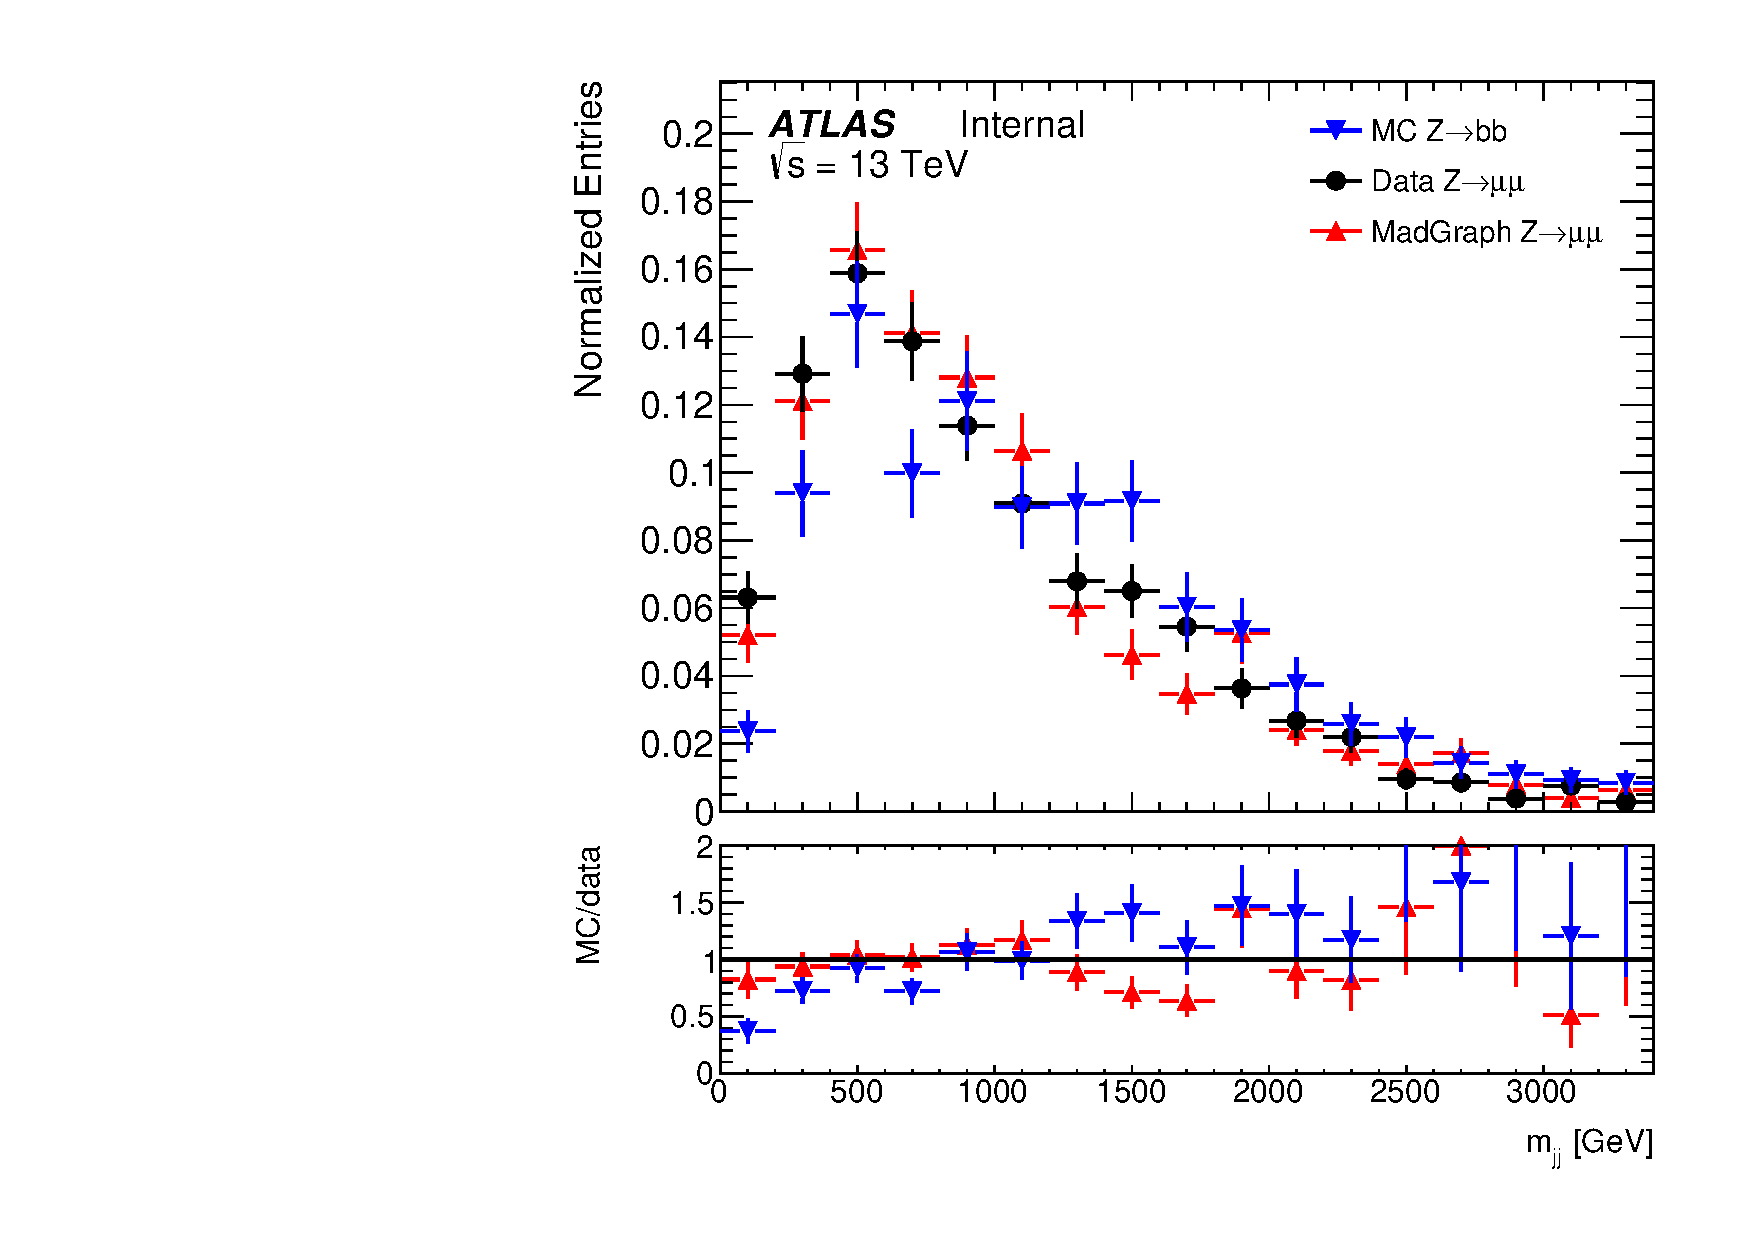
\includegraphics[width=0.3\textwidth]{figures/Zmumu/BDTinput_2j_hmJJ.pdf}
 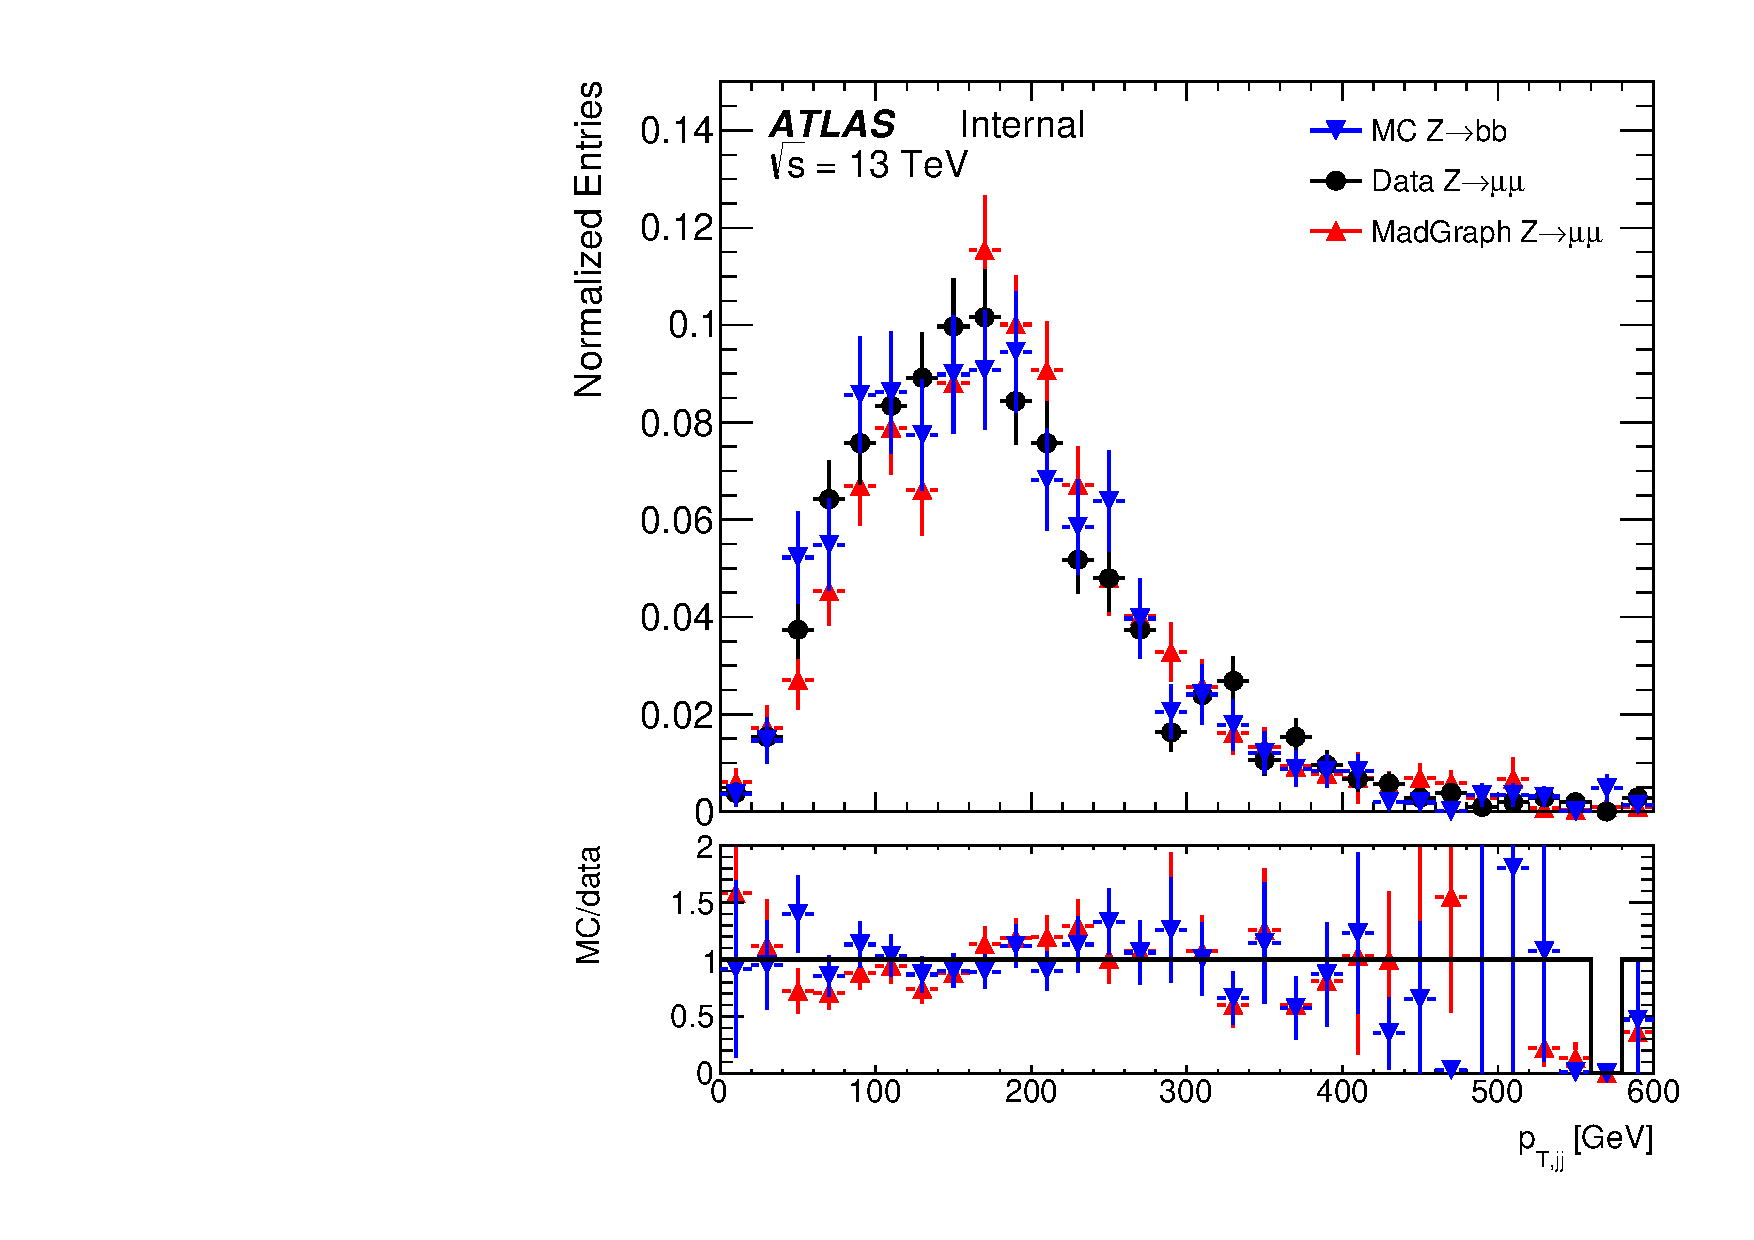
\includegraphics[width=0.3\textwidth]{figures/Zmumu/BDTinput_2j_hpTJJ.pdf}
 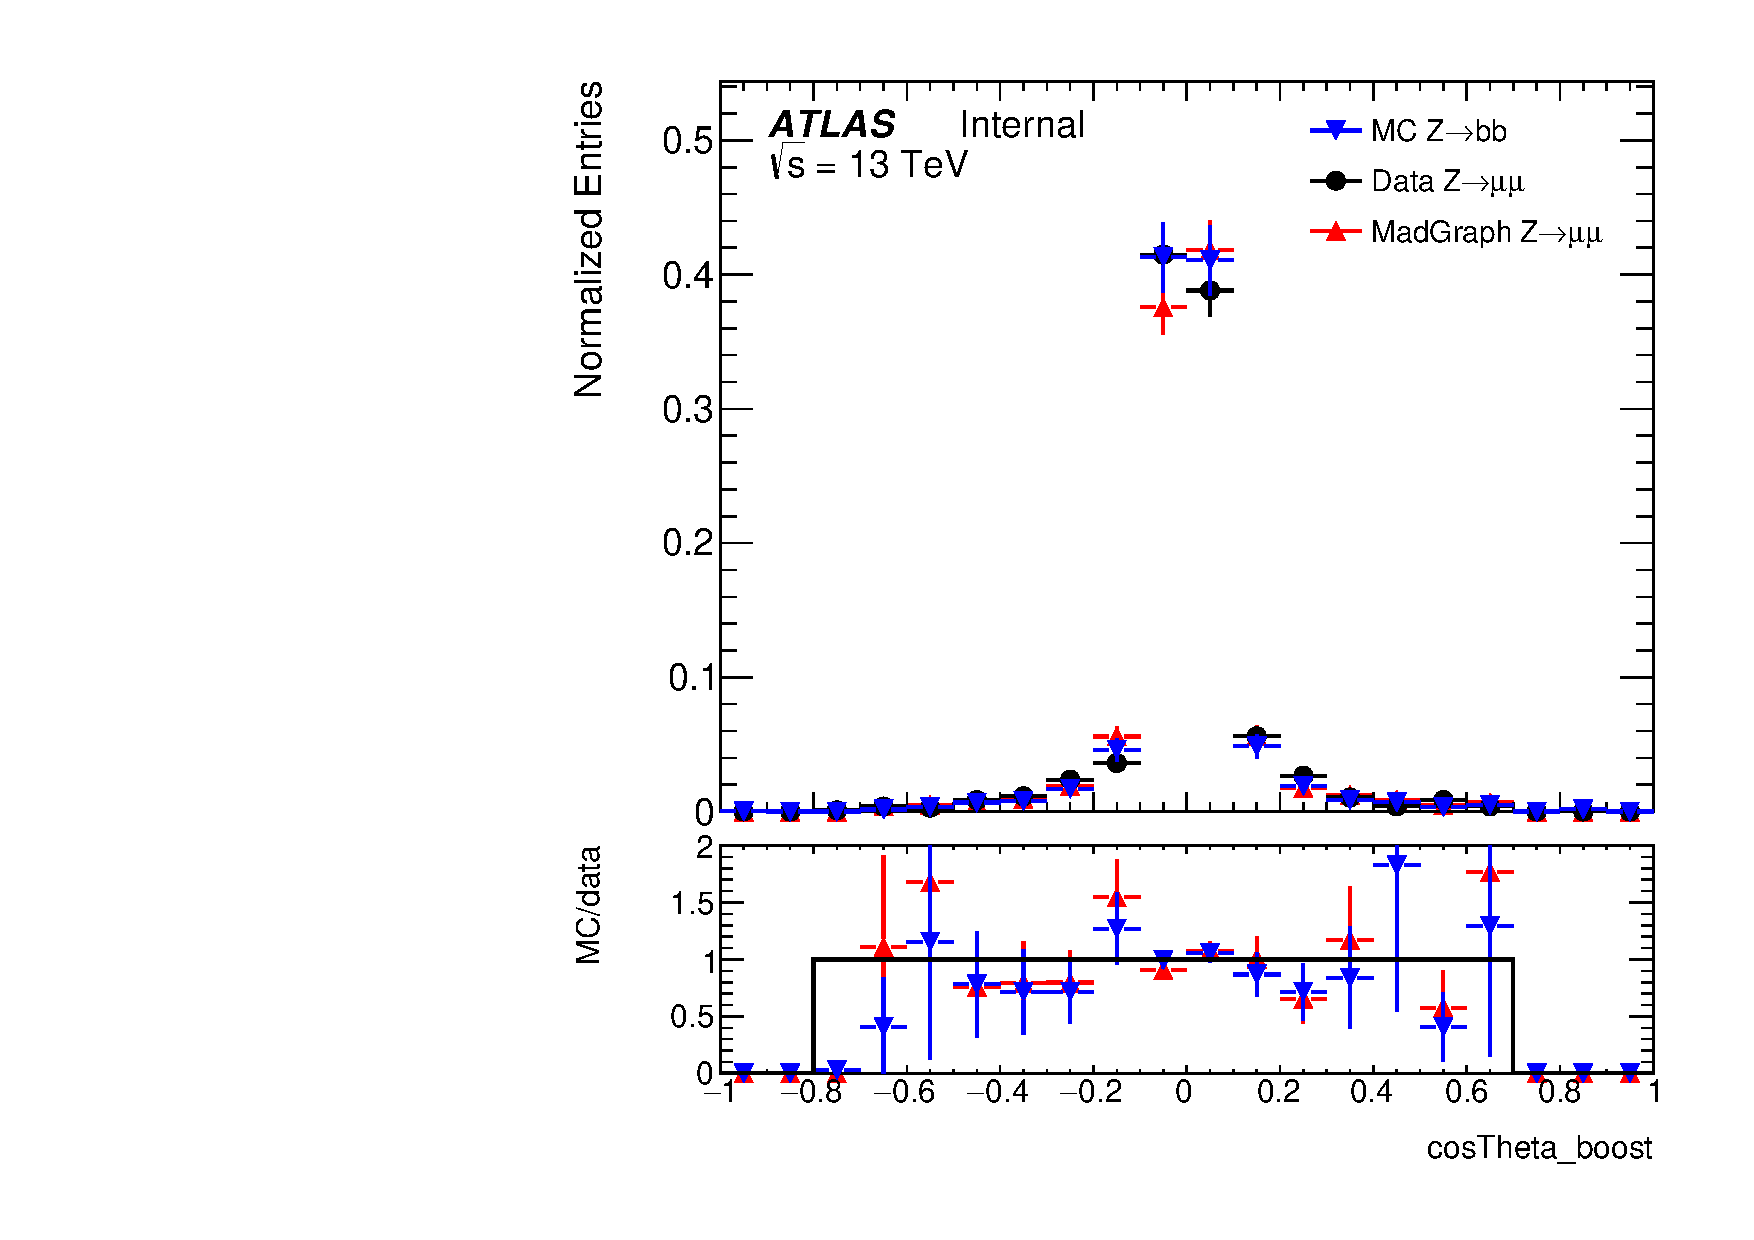
\includegraphics[width=0.3\textwidth]{figures/Zmumu/BDTinput_2j_hcosTheta_boost.pdf}\\
 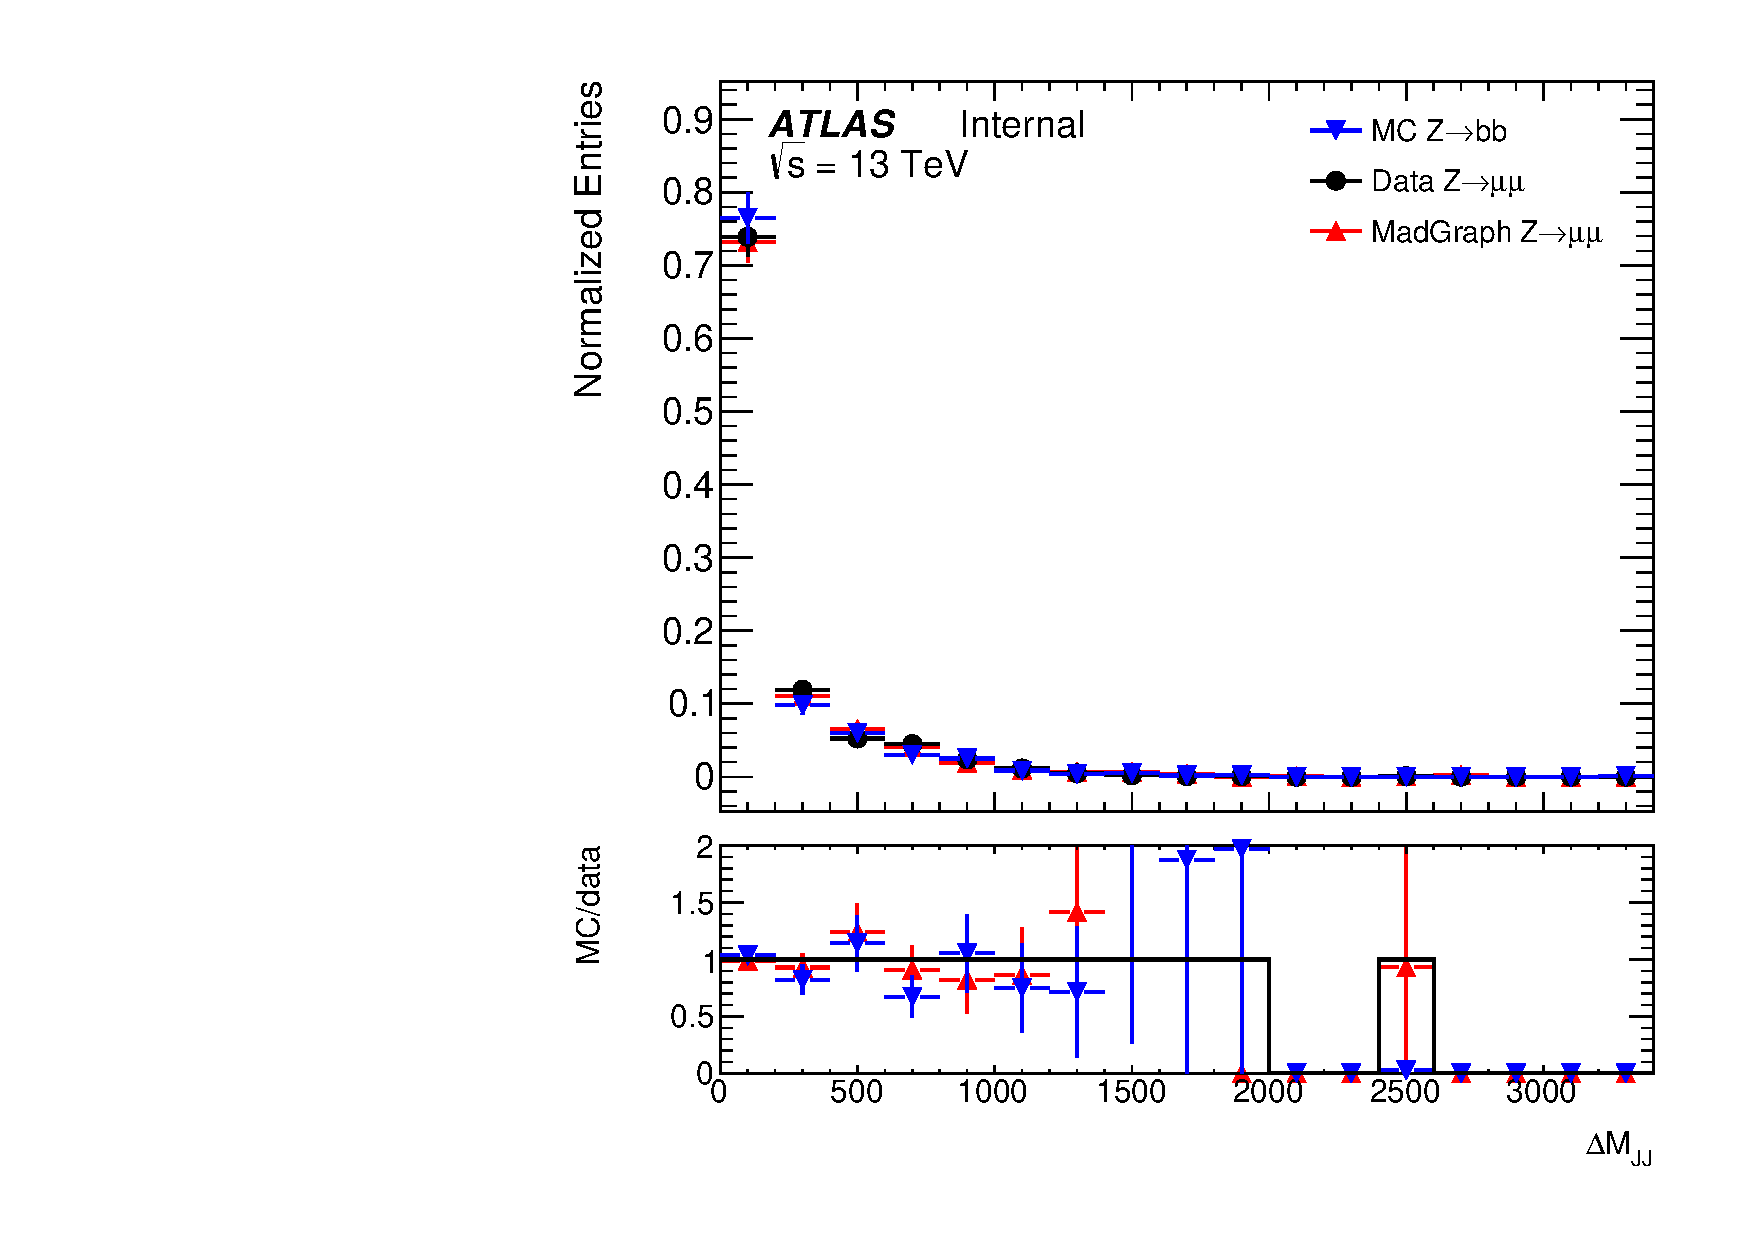
\includegraphics[width=0.3\textwidth]{figures/Zmumu/BDTinput_2j_hdeltaMJJ.pdf}
 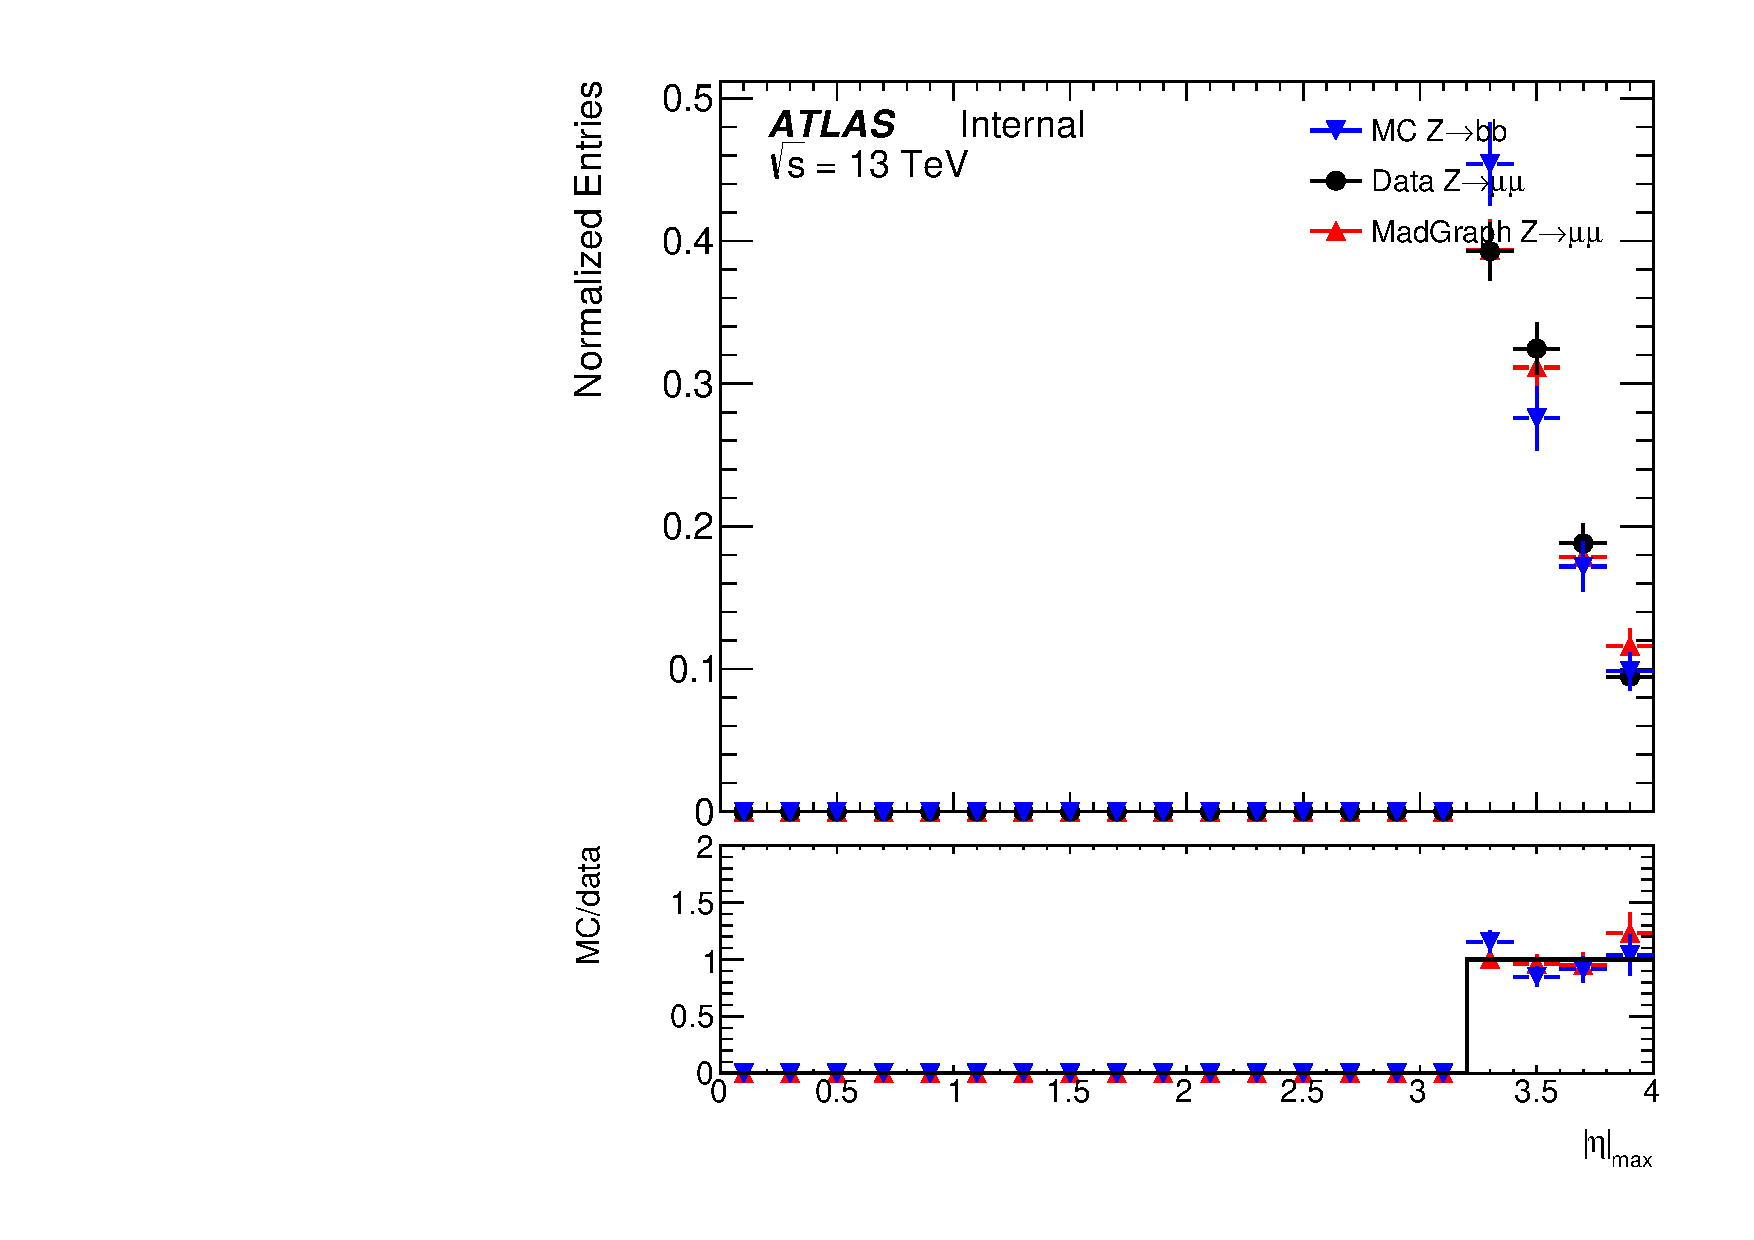
\includegraphics[width=0.3\textwidth]{figures/Zmumu/BDTinput_2j_hmax_J1J2.pdf}
 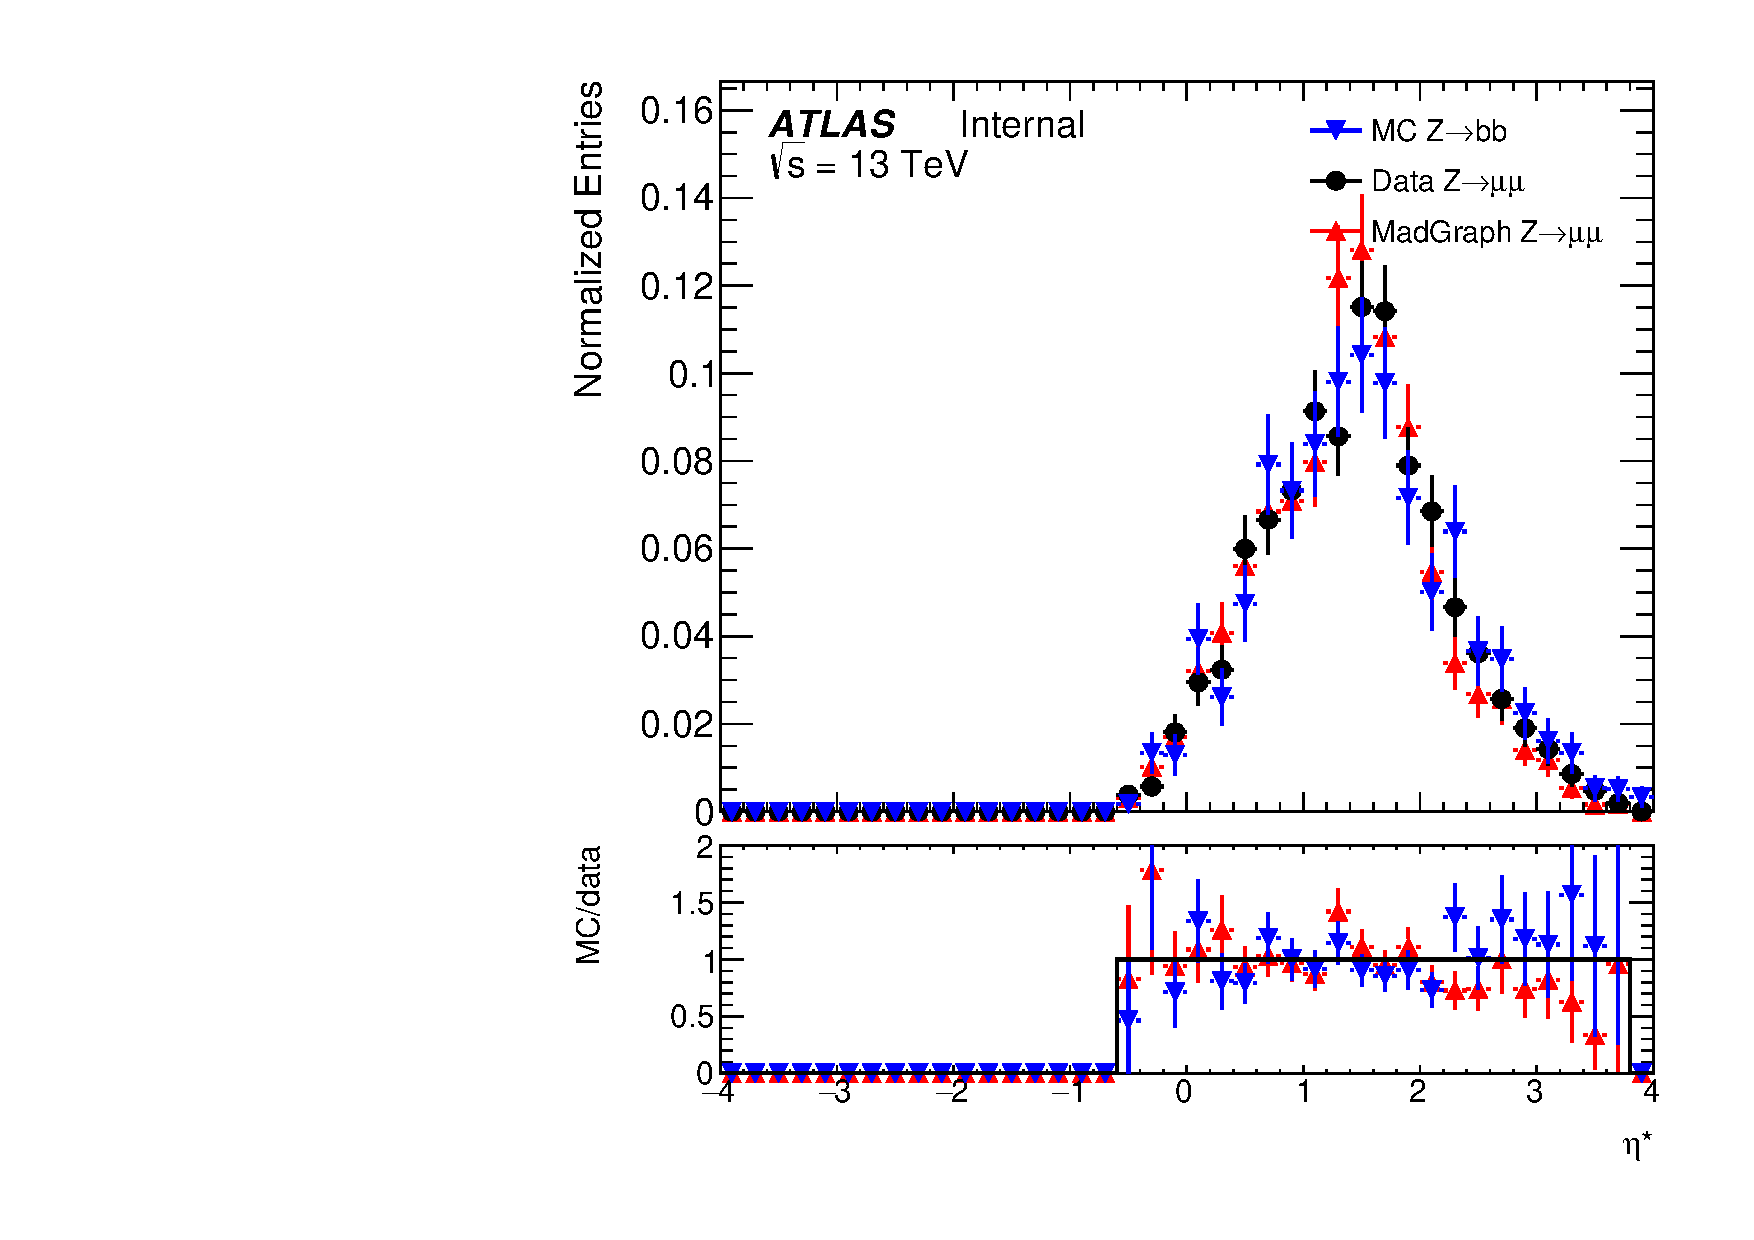
\includegraphics[width=0.3\textwidth]{figures/Zmumu/BDTinput_2j_heta_J_star.pdf}\\
 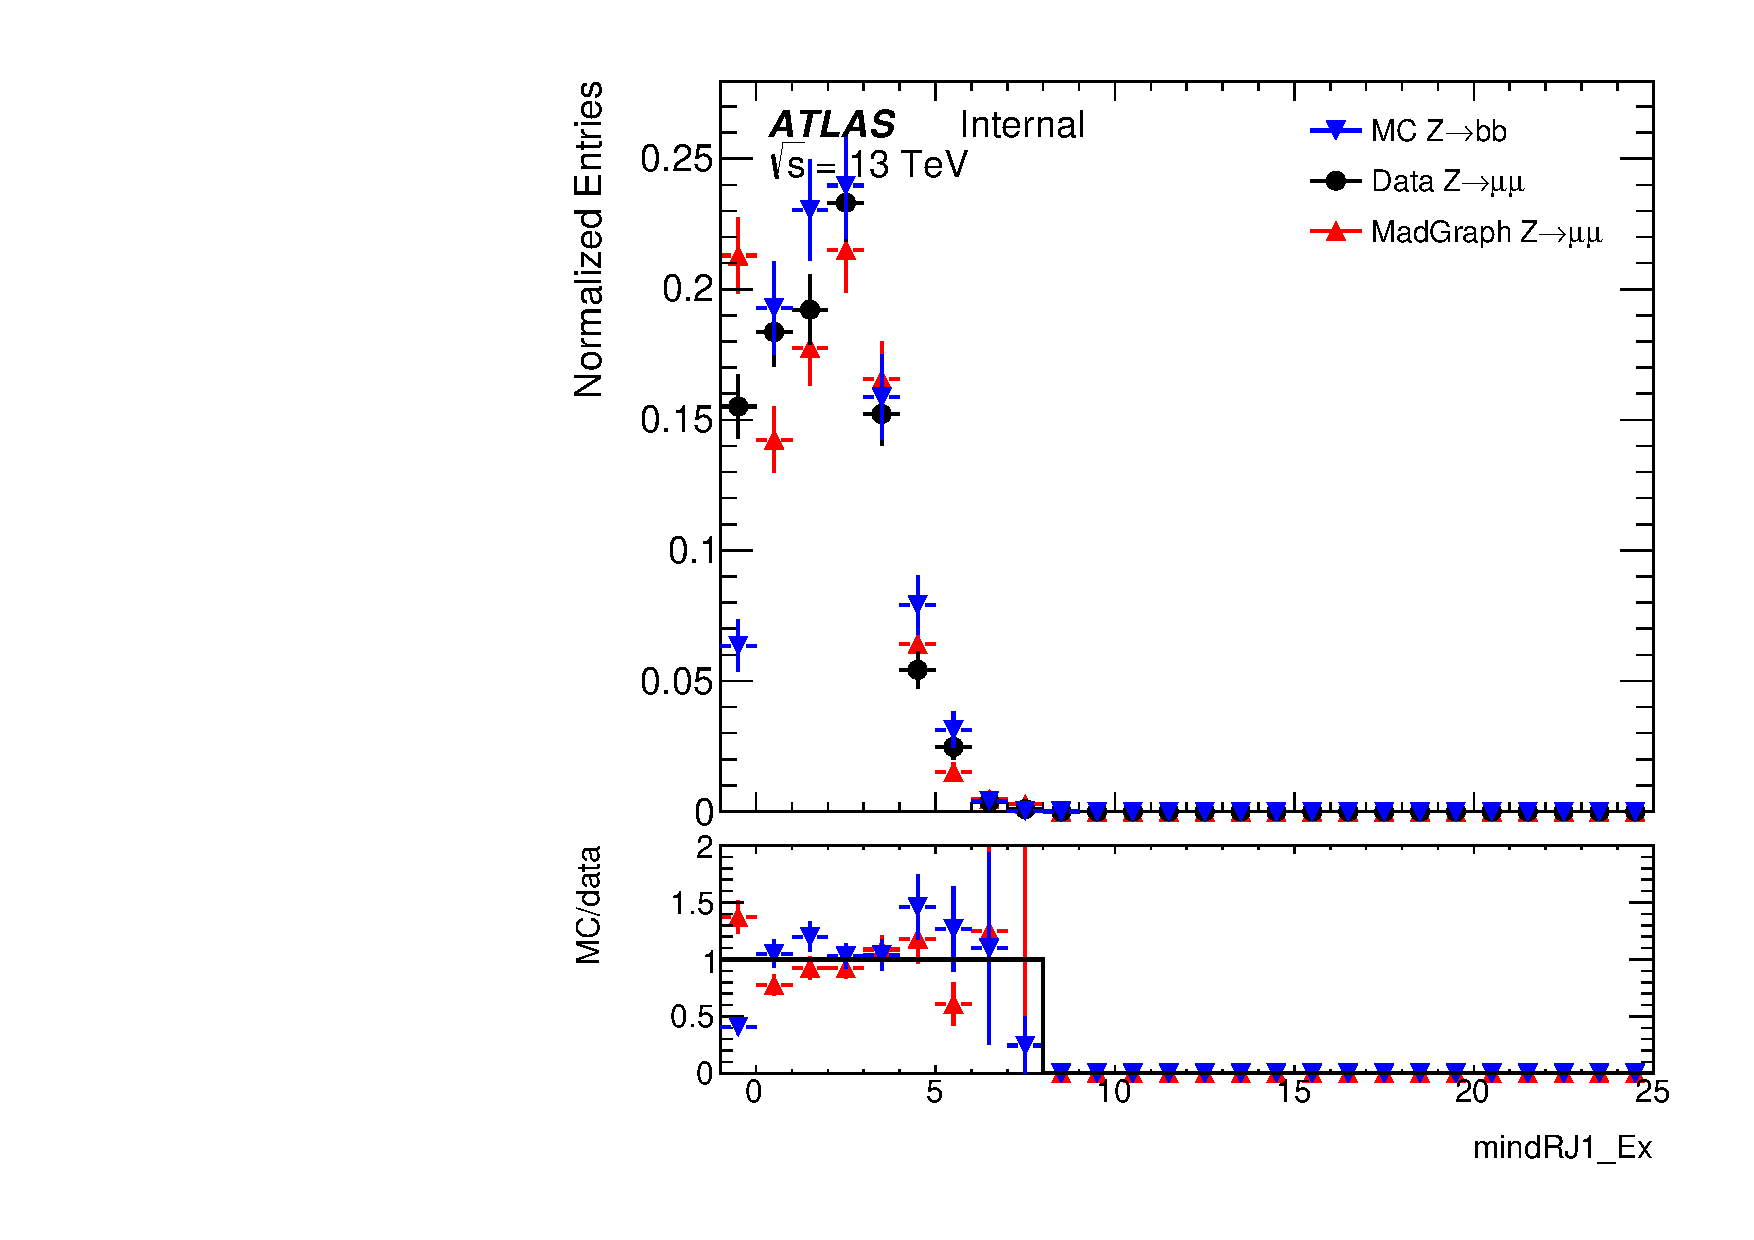
\includegraphics[width=0.3\textwidth]{figures/Zmumu/BDTinput_2j_hmindRJ1_Ex.pdf}
 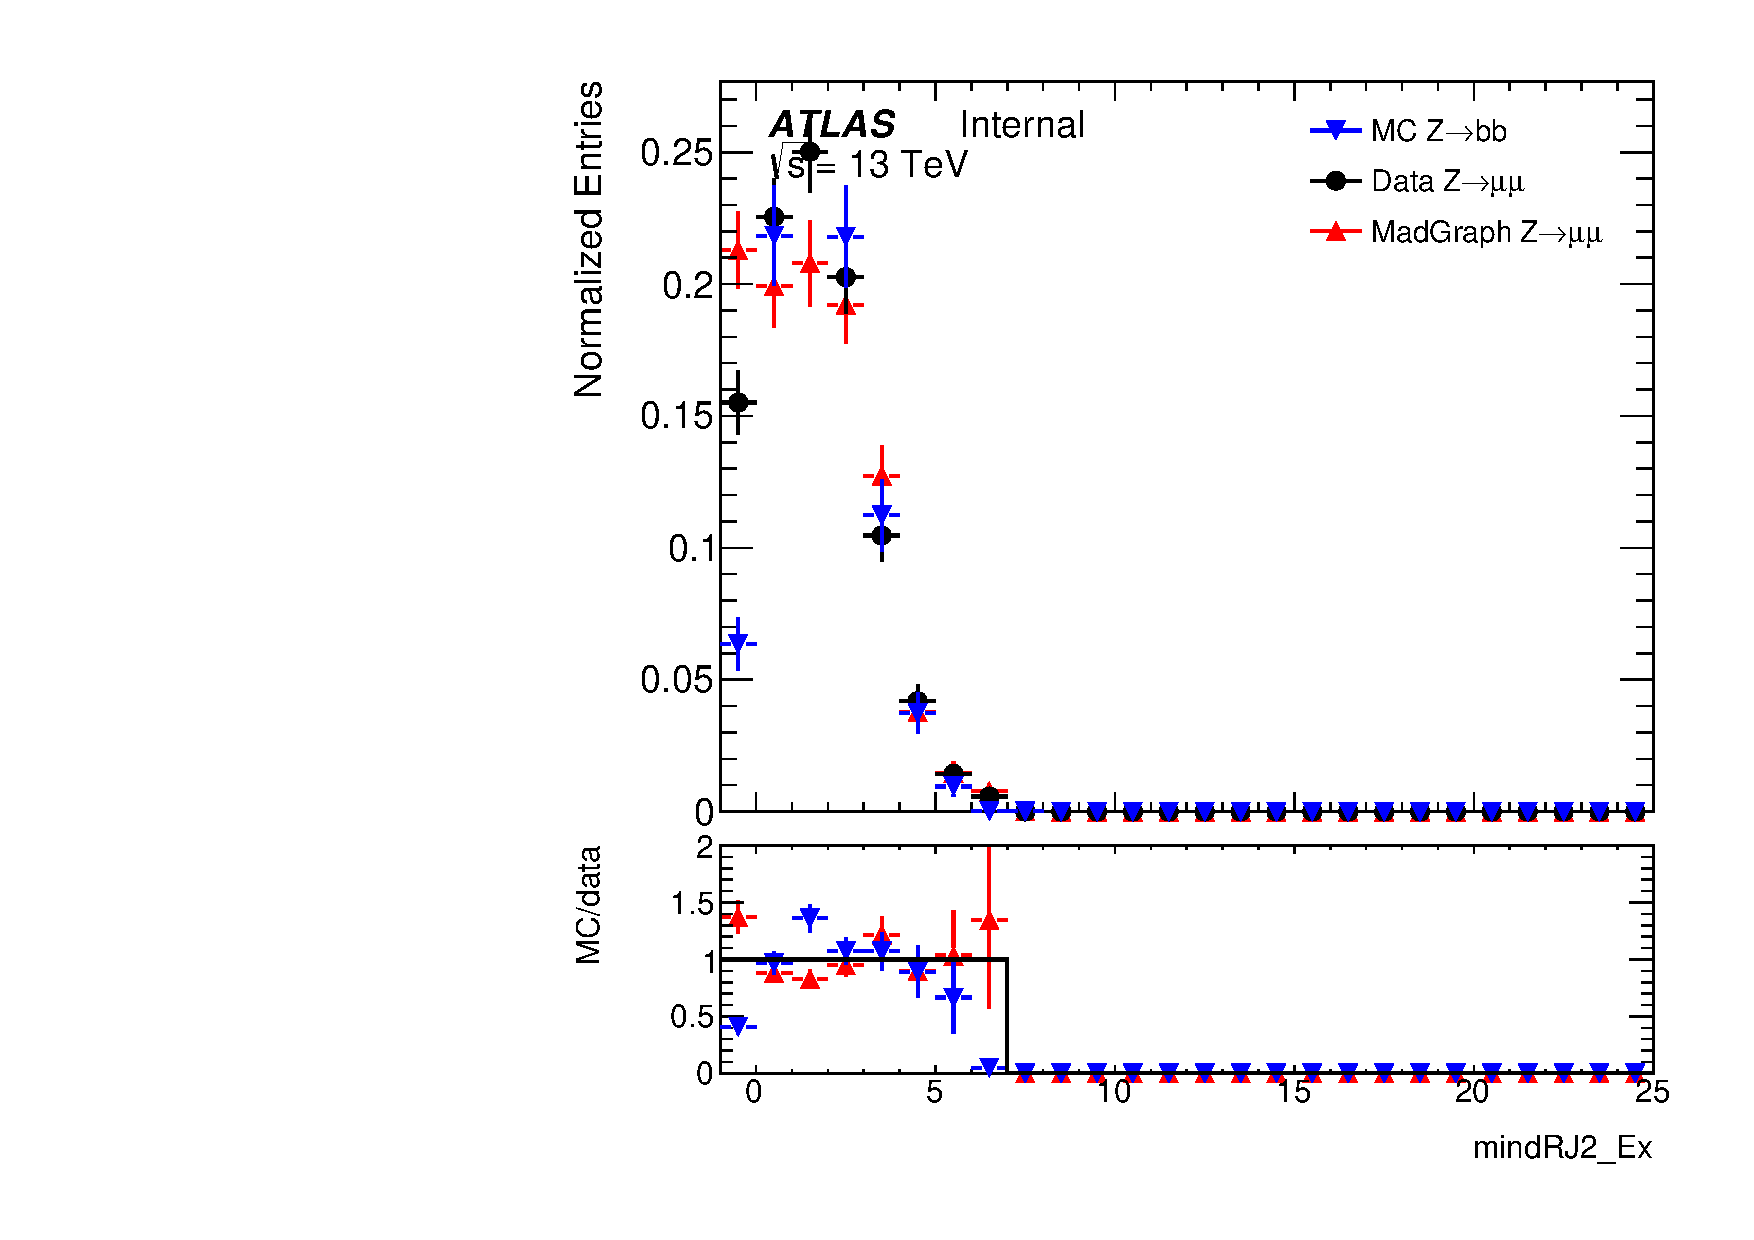
\includegraphics[width=0.3\textwidth]{figures/Zmumu/BDTinput_2j_hmindRJ2_Ex.pdf}
 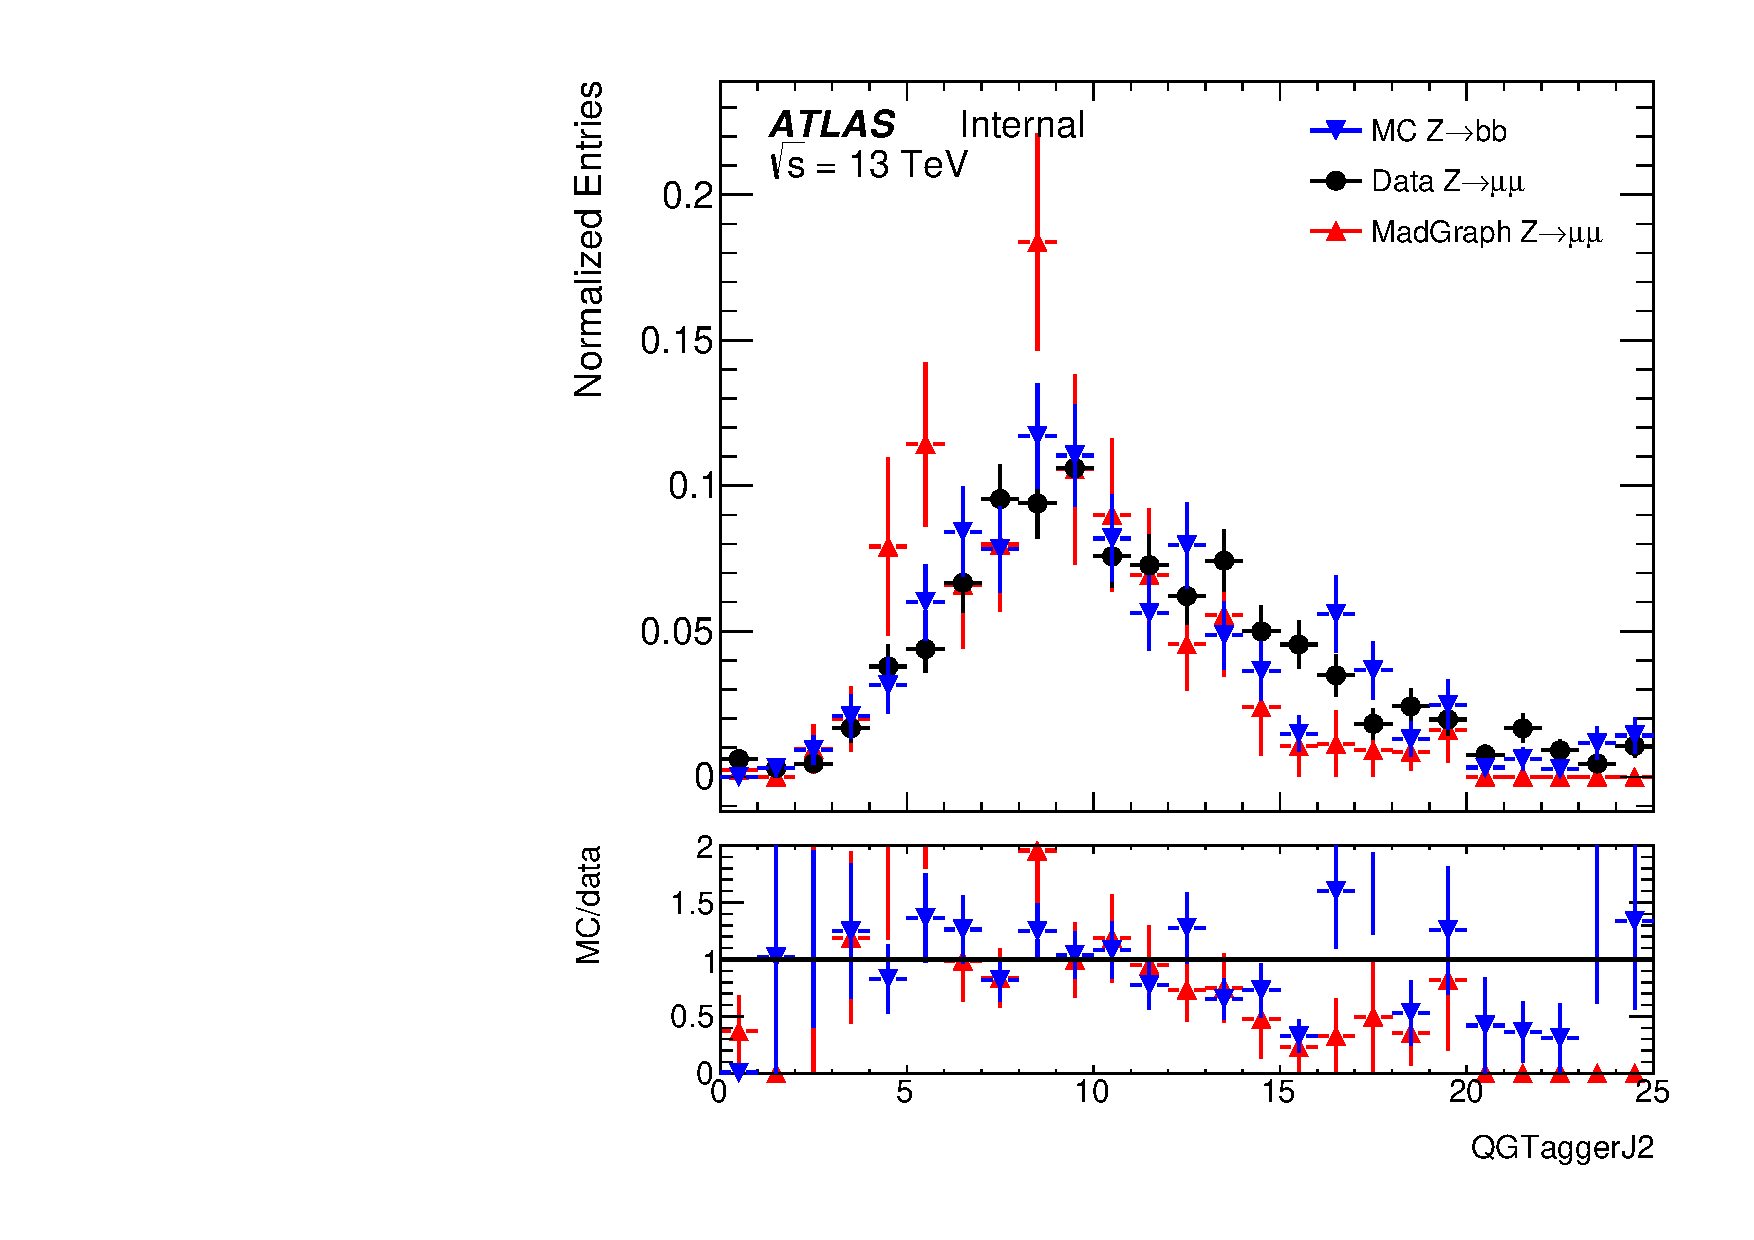
\includegraphics[width=0.3\textwidth]{figures/Zmumu/BDTinput_2j_hQGTaggerJ2.pdf}\\
 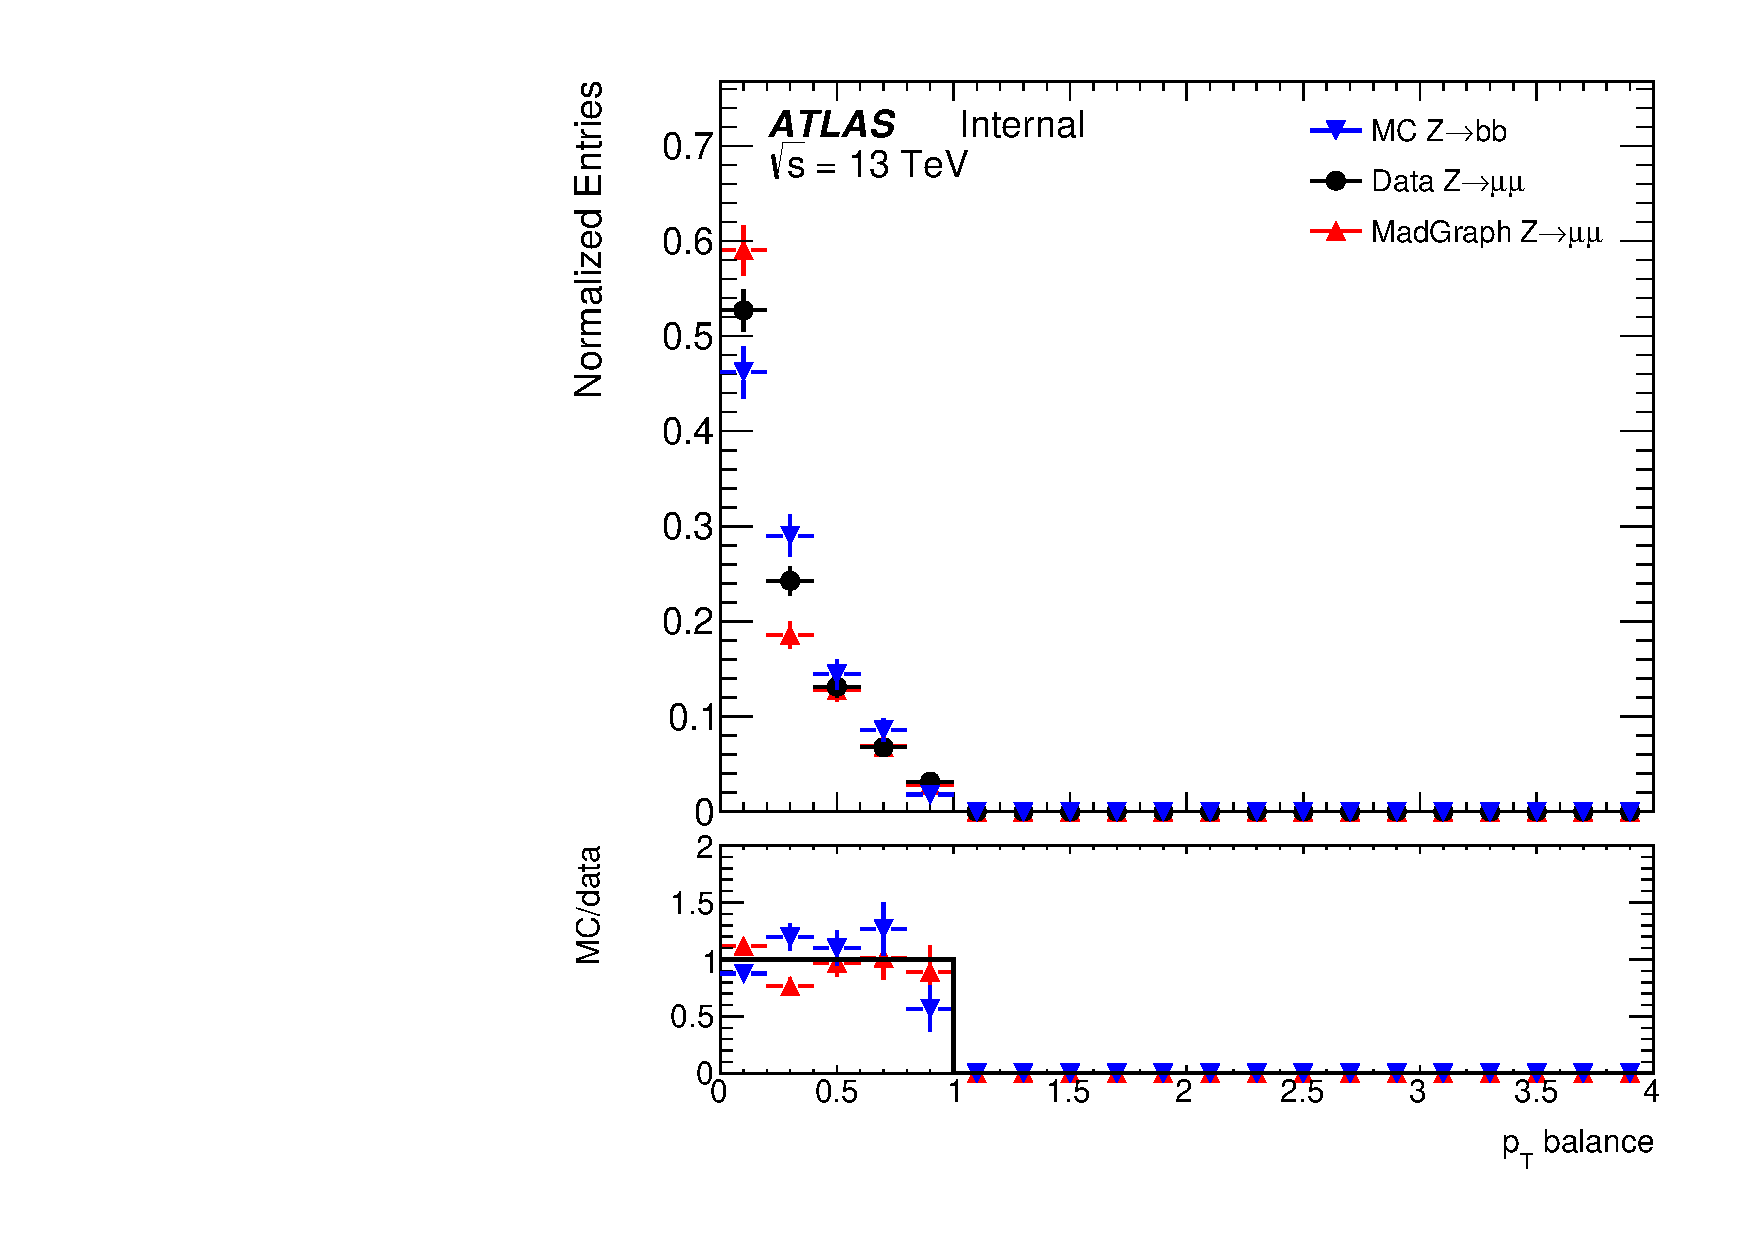
\includegraphics[width=0.3\textwidth]{figures/Zmumu/BDTinput_2j_hpT_balance.pdf}\\
\caption{Distributions of BDT input variables of \twocentral channel.  $N_{\rm Trk}($J1$)PV500$ is identically zero because J1 is by definition outside of the tracker acceptance.}
  \label{fig:ZmmBDTInputs2cen}
\end{figure}

\begin{figure}[htbp]
  \centering
 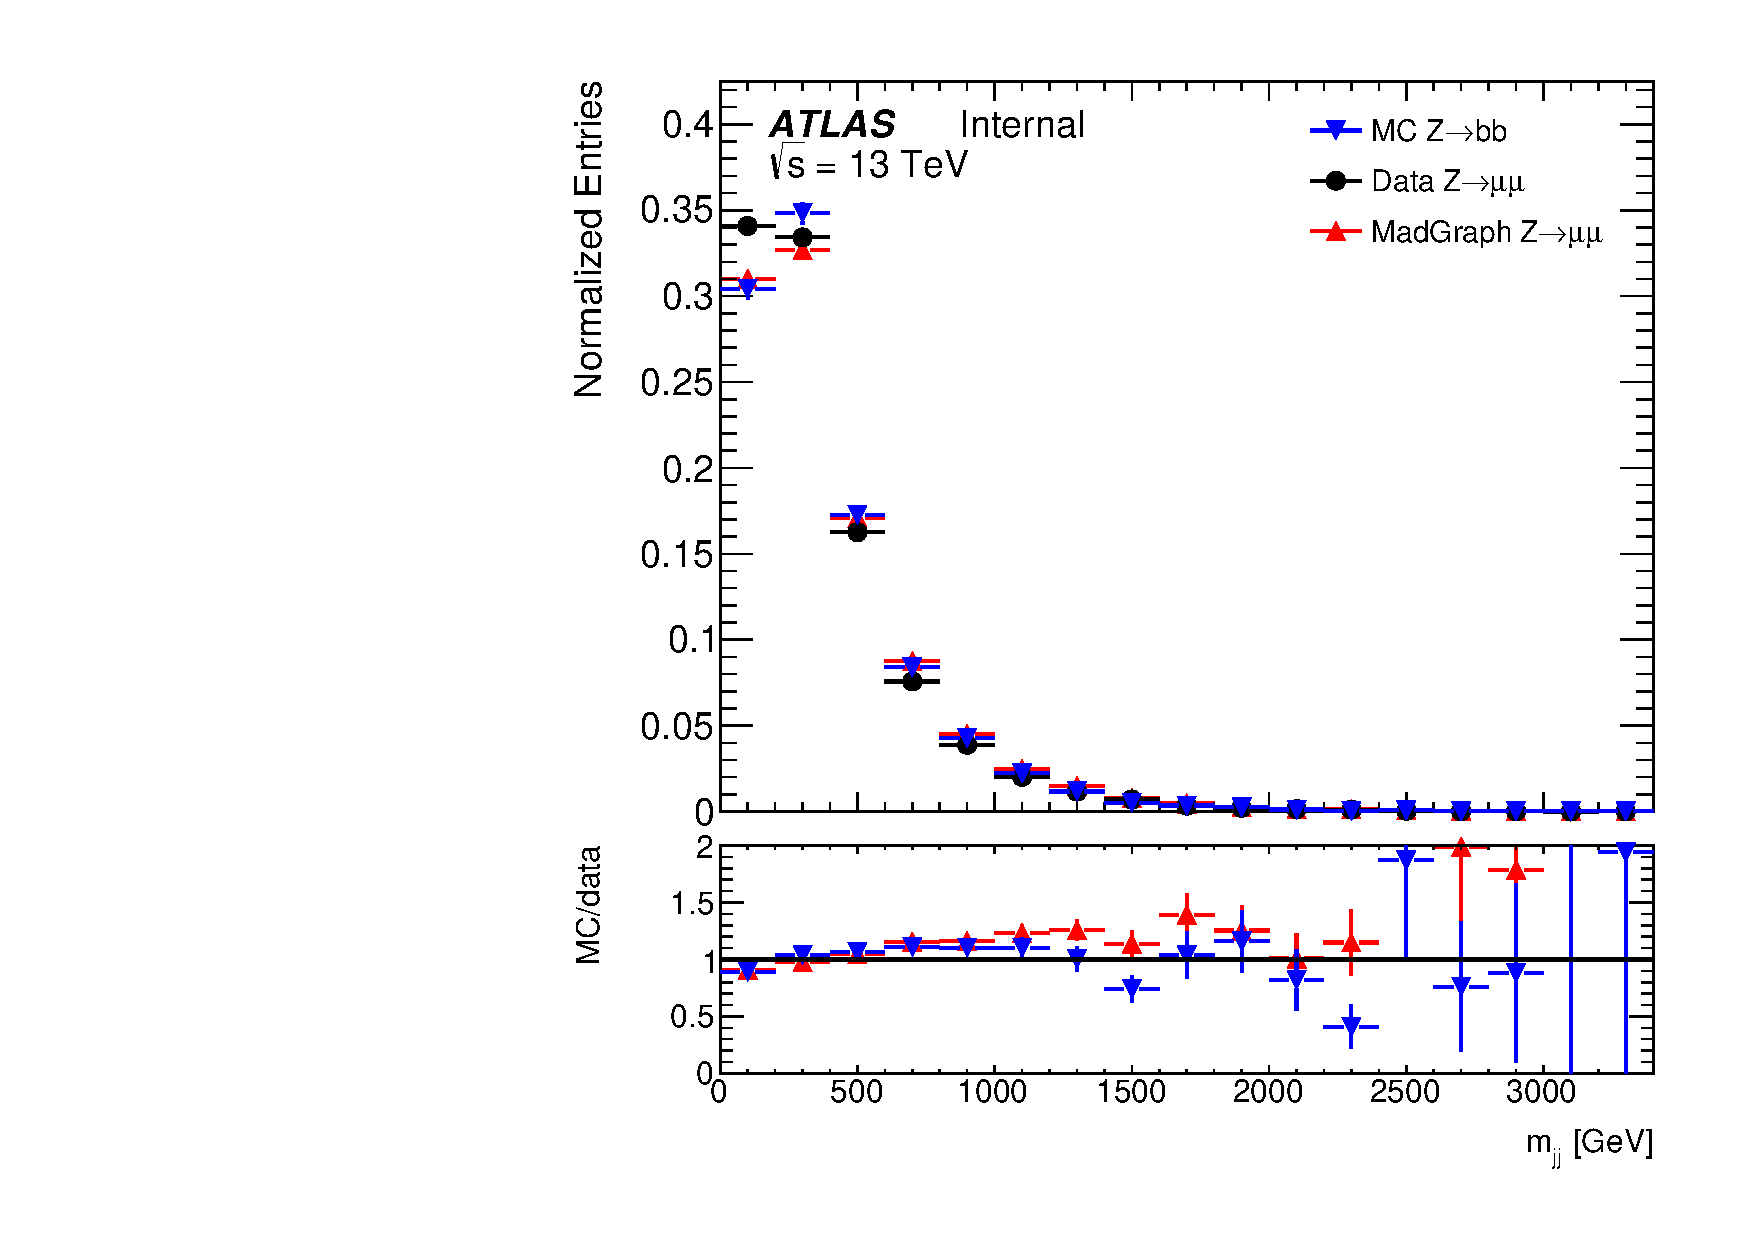
\includegraphics[width=0.3\textwidth]{figures/Zmumu/BDTinput_hmJJ.pdf}
 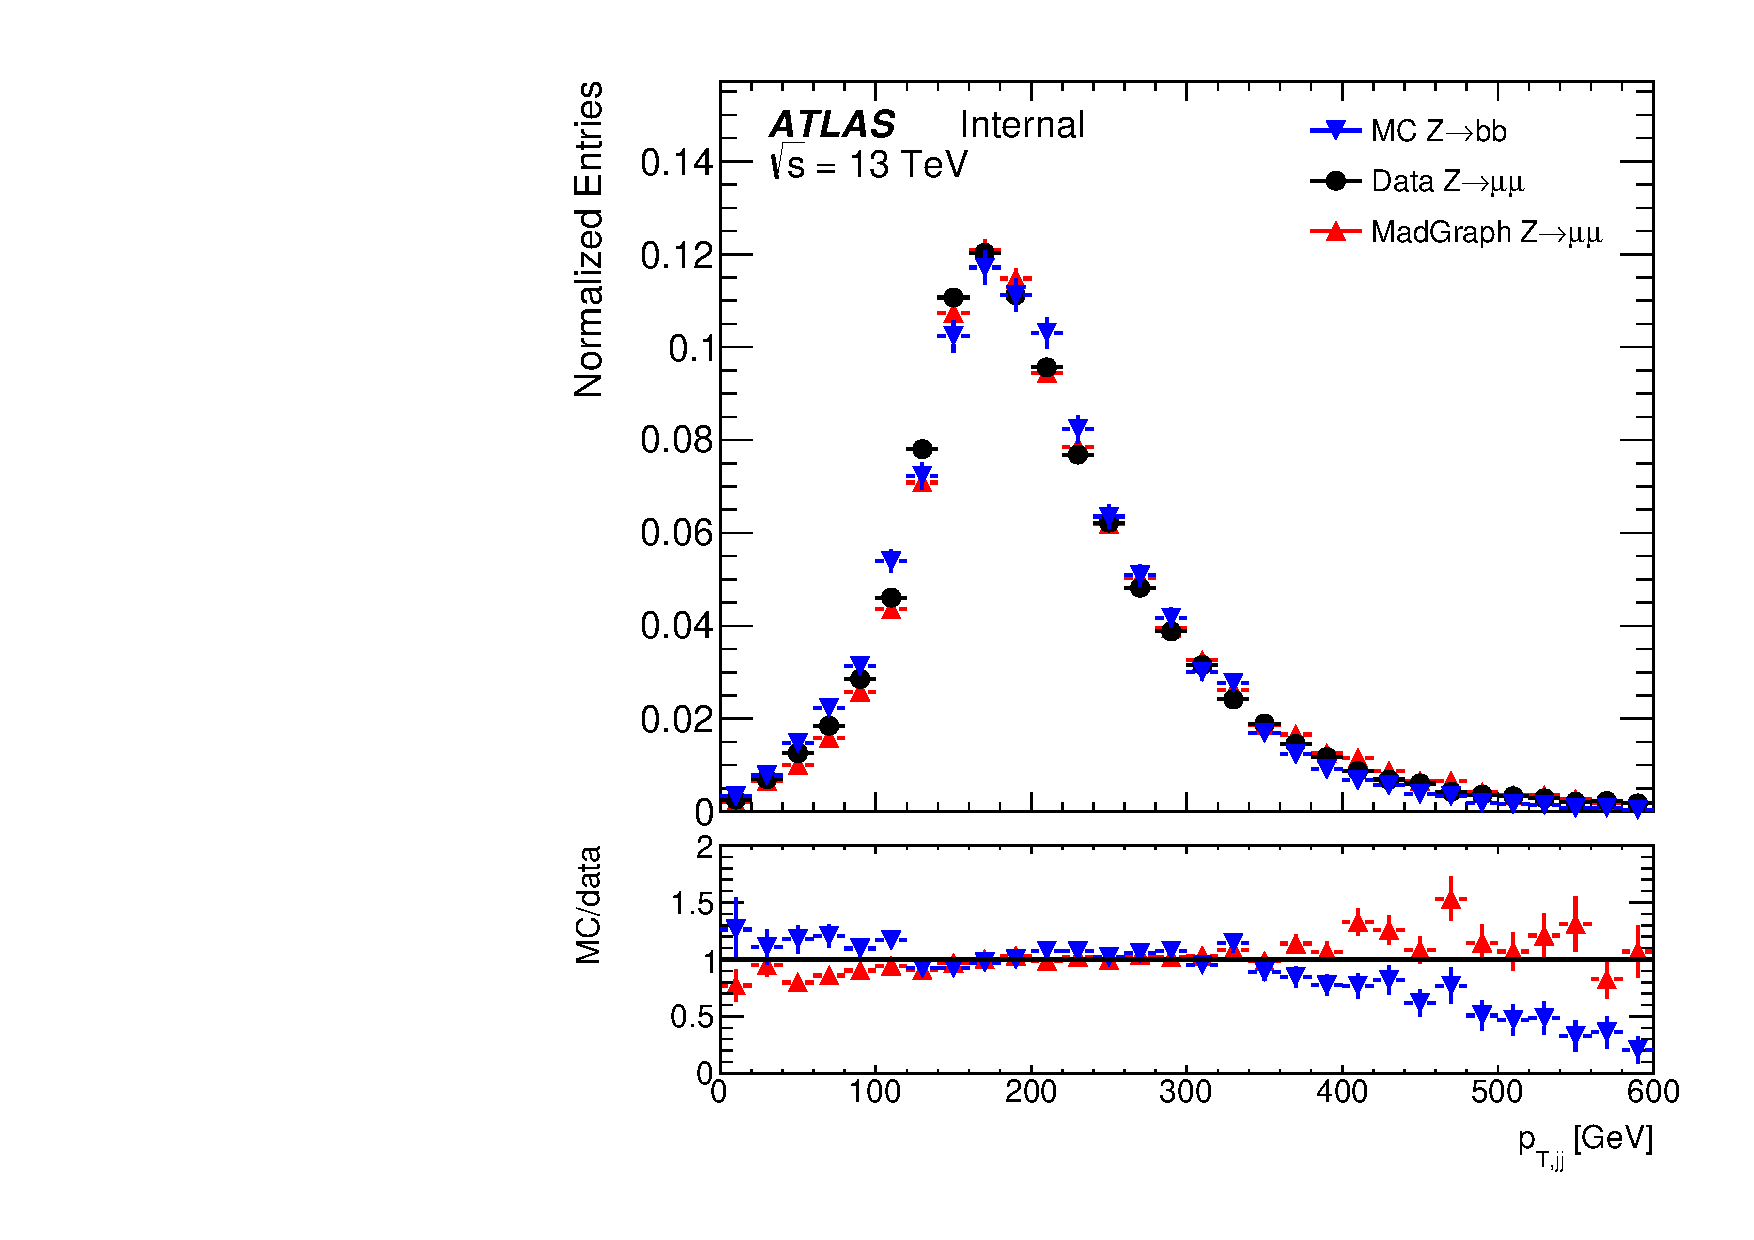
\includegraphics[width=0.3\textwidth]{figures/Zmumu/BDTinput_hpTJJ.pdf}
 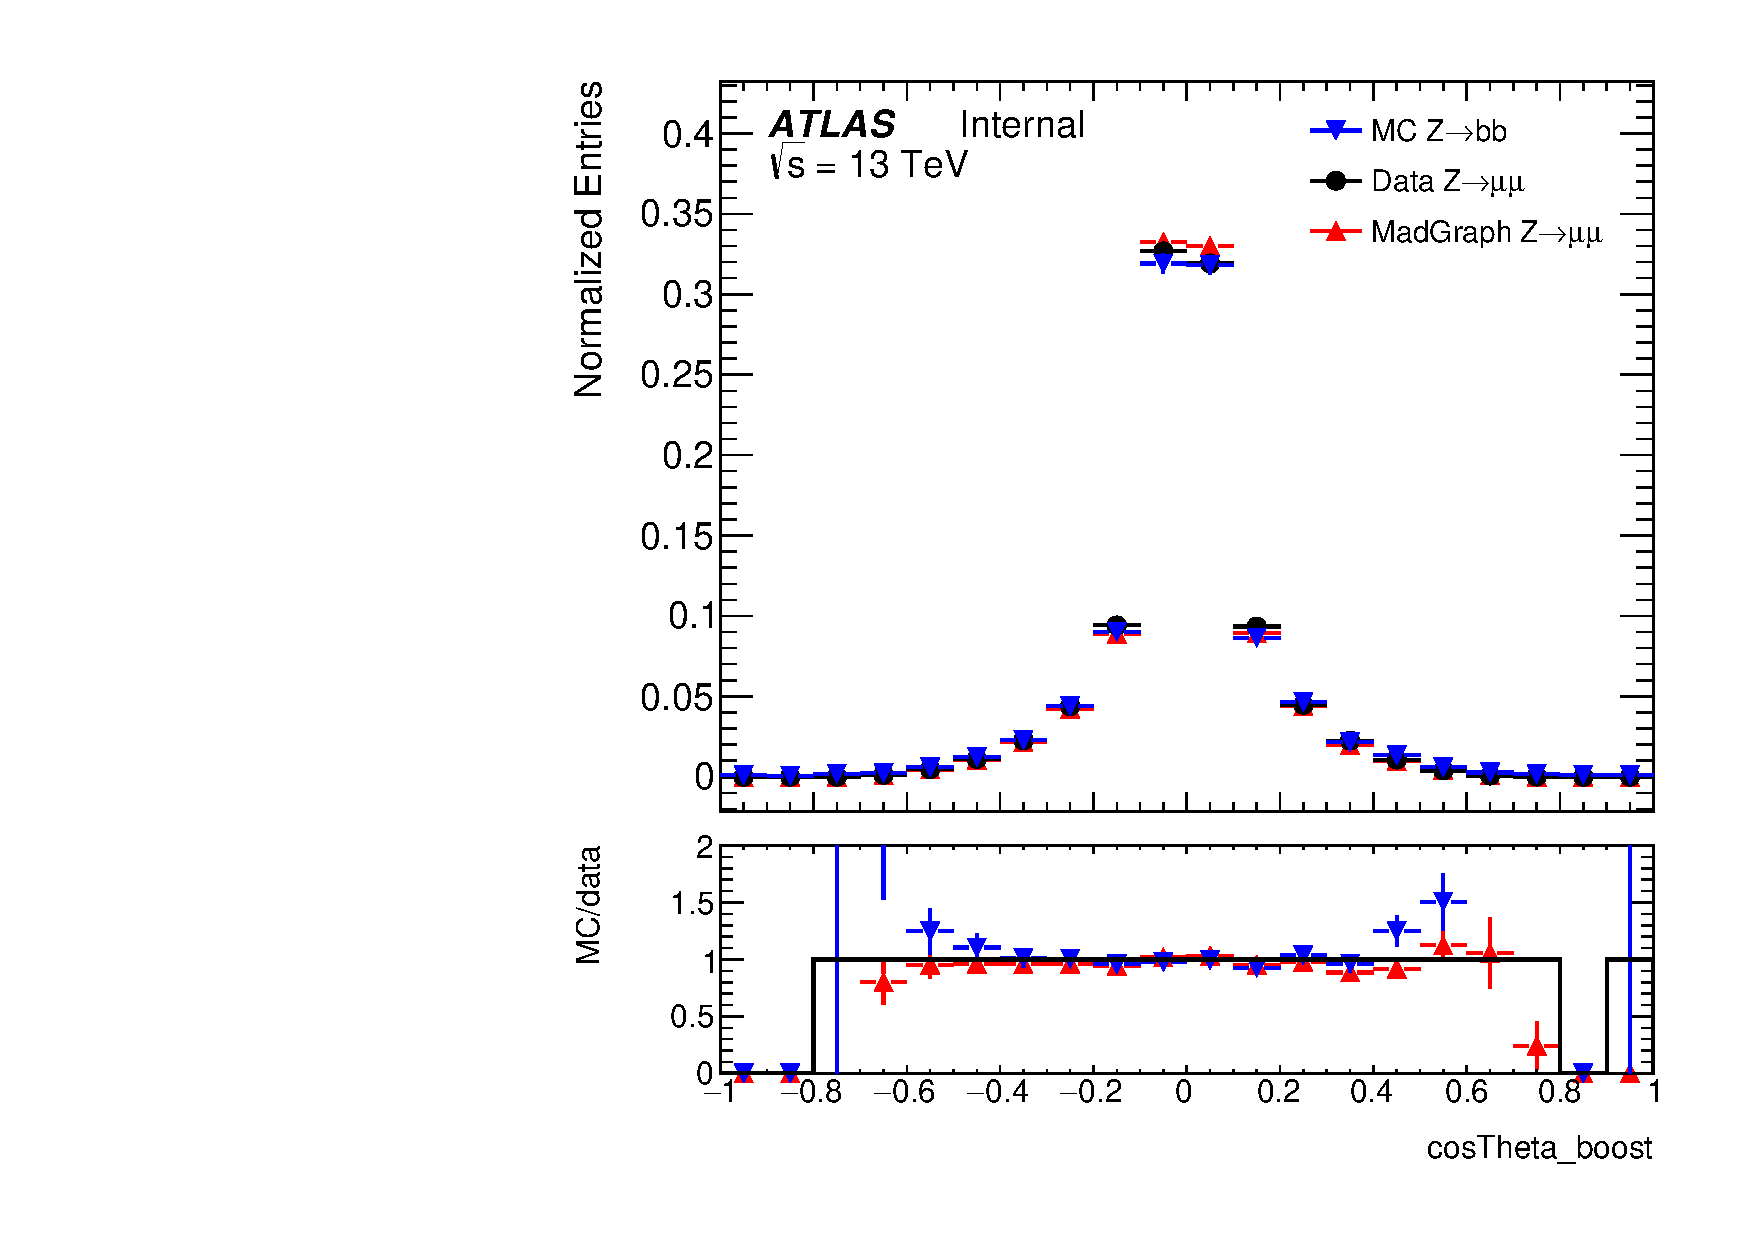
\includegraphics[width=0.3\textwidth]{figures/Zmumu/BDTinput_hcosTheta_boost.pdf}\\
 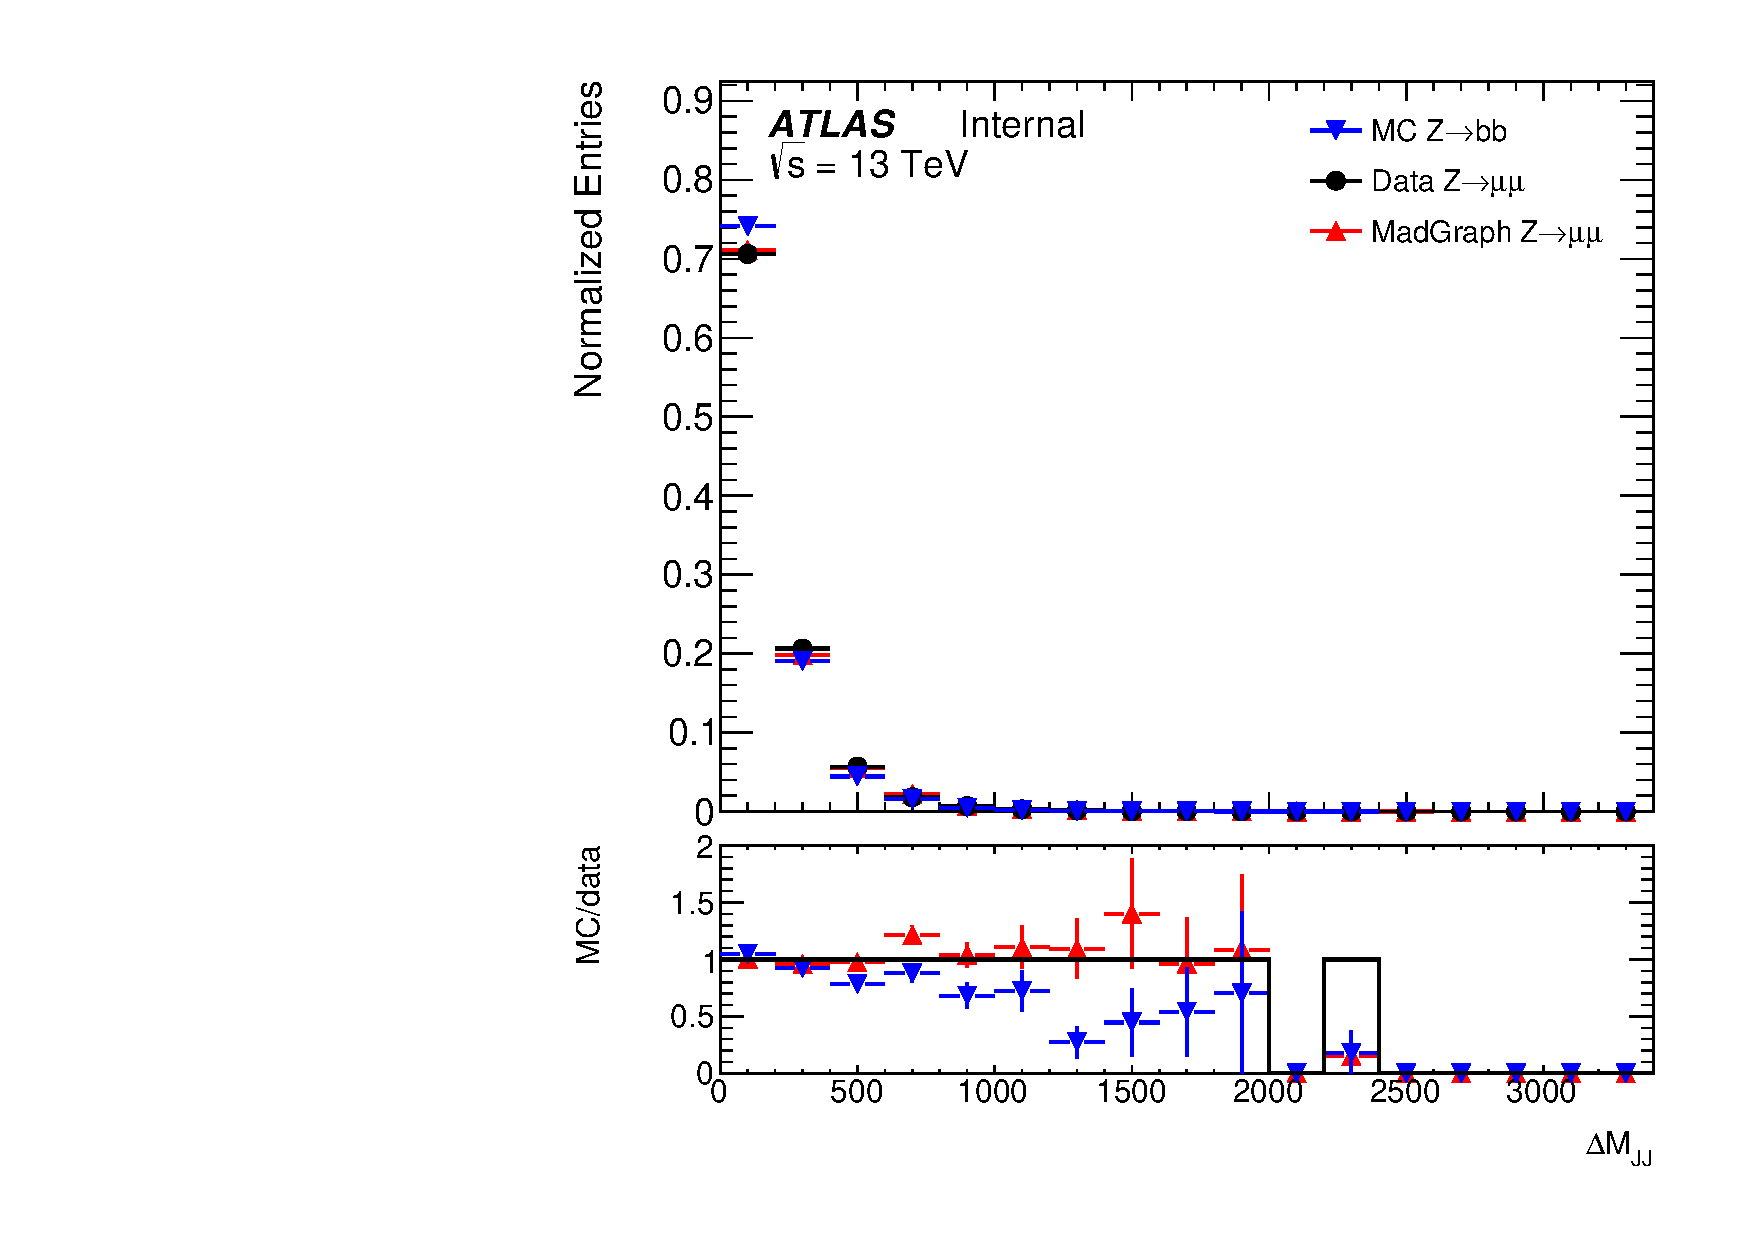
\includegraphics[width=0.3\textwidth]{figures/Zmumu/BDTinput_hdeltaMJJ.pdf}
 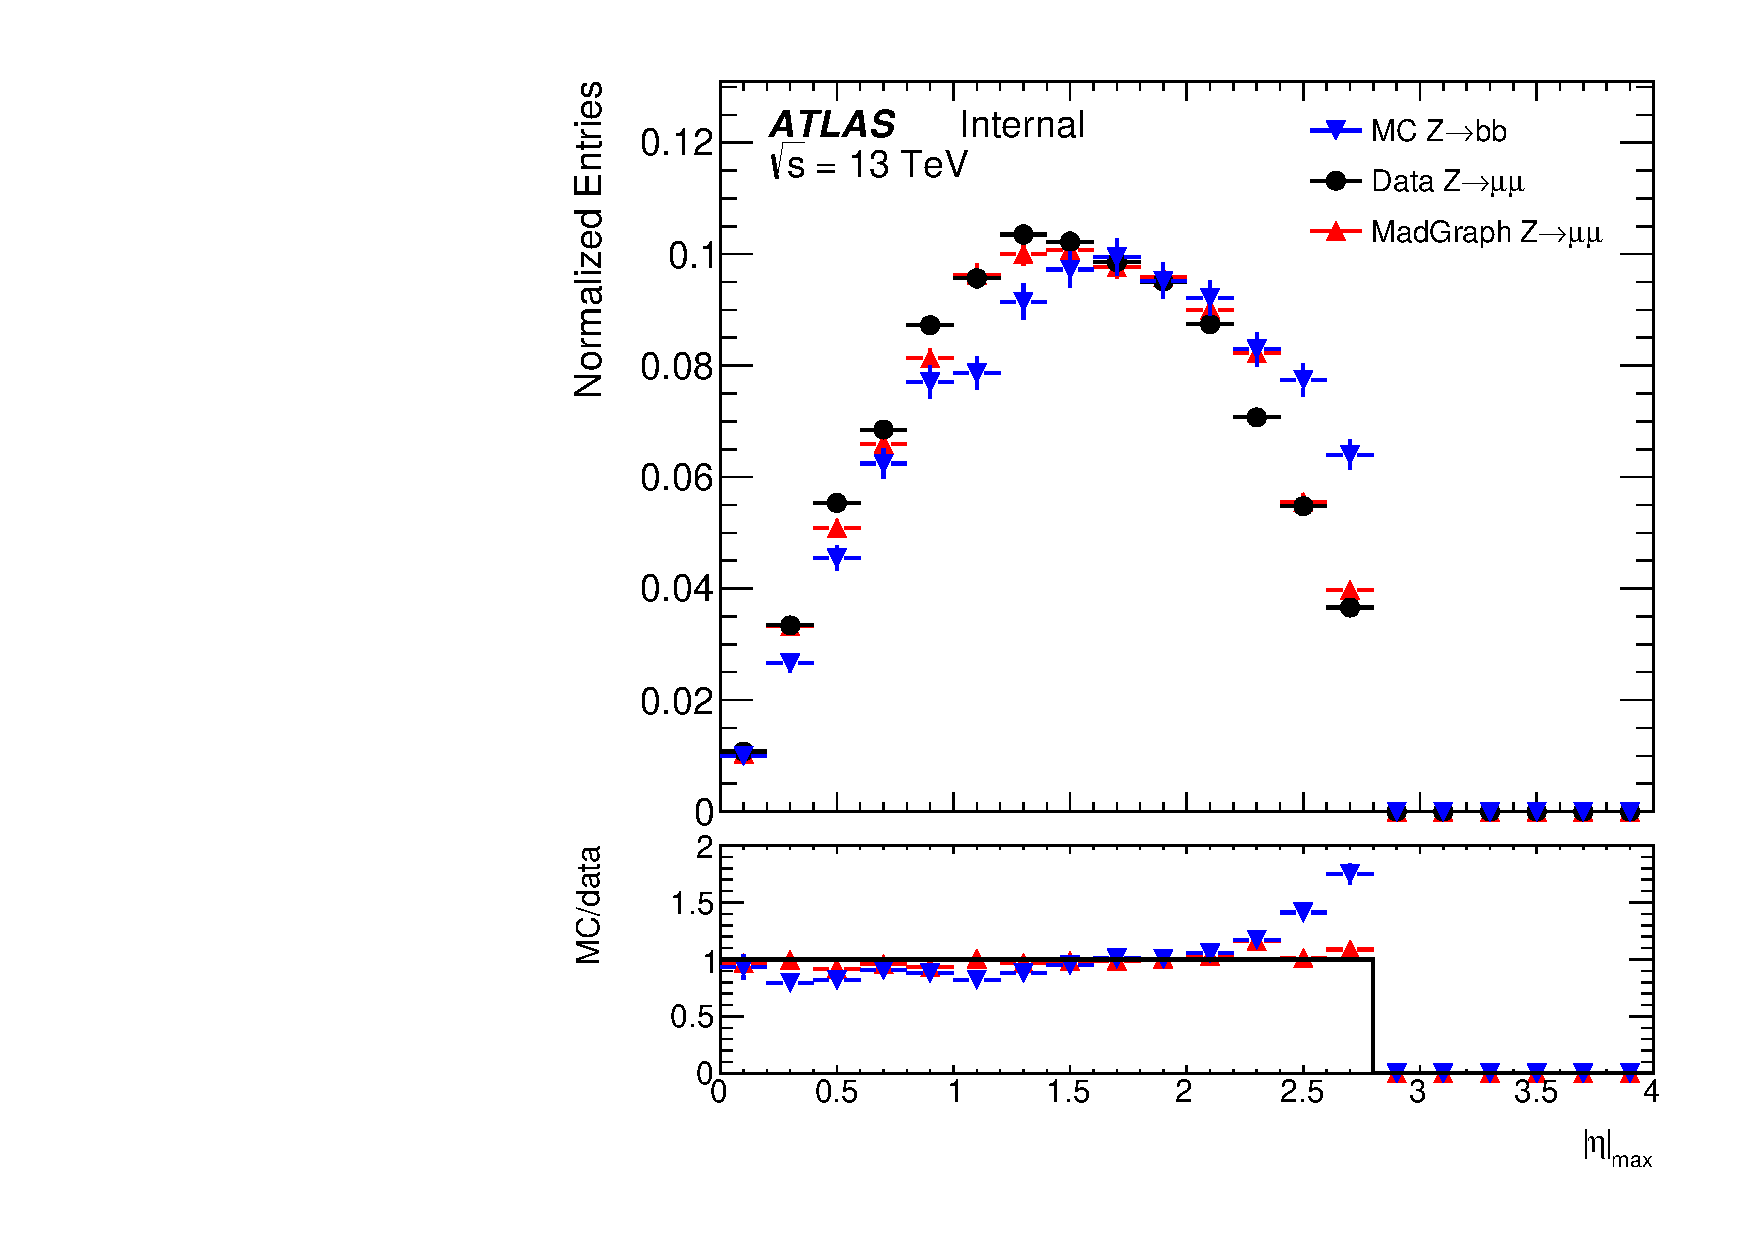
\includegraphics[width=0.3\textwidth]{figures/Zmumu/BDTinput_hmax_J1J2.pdf}
 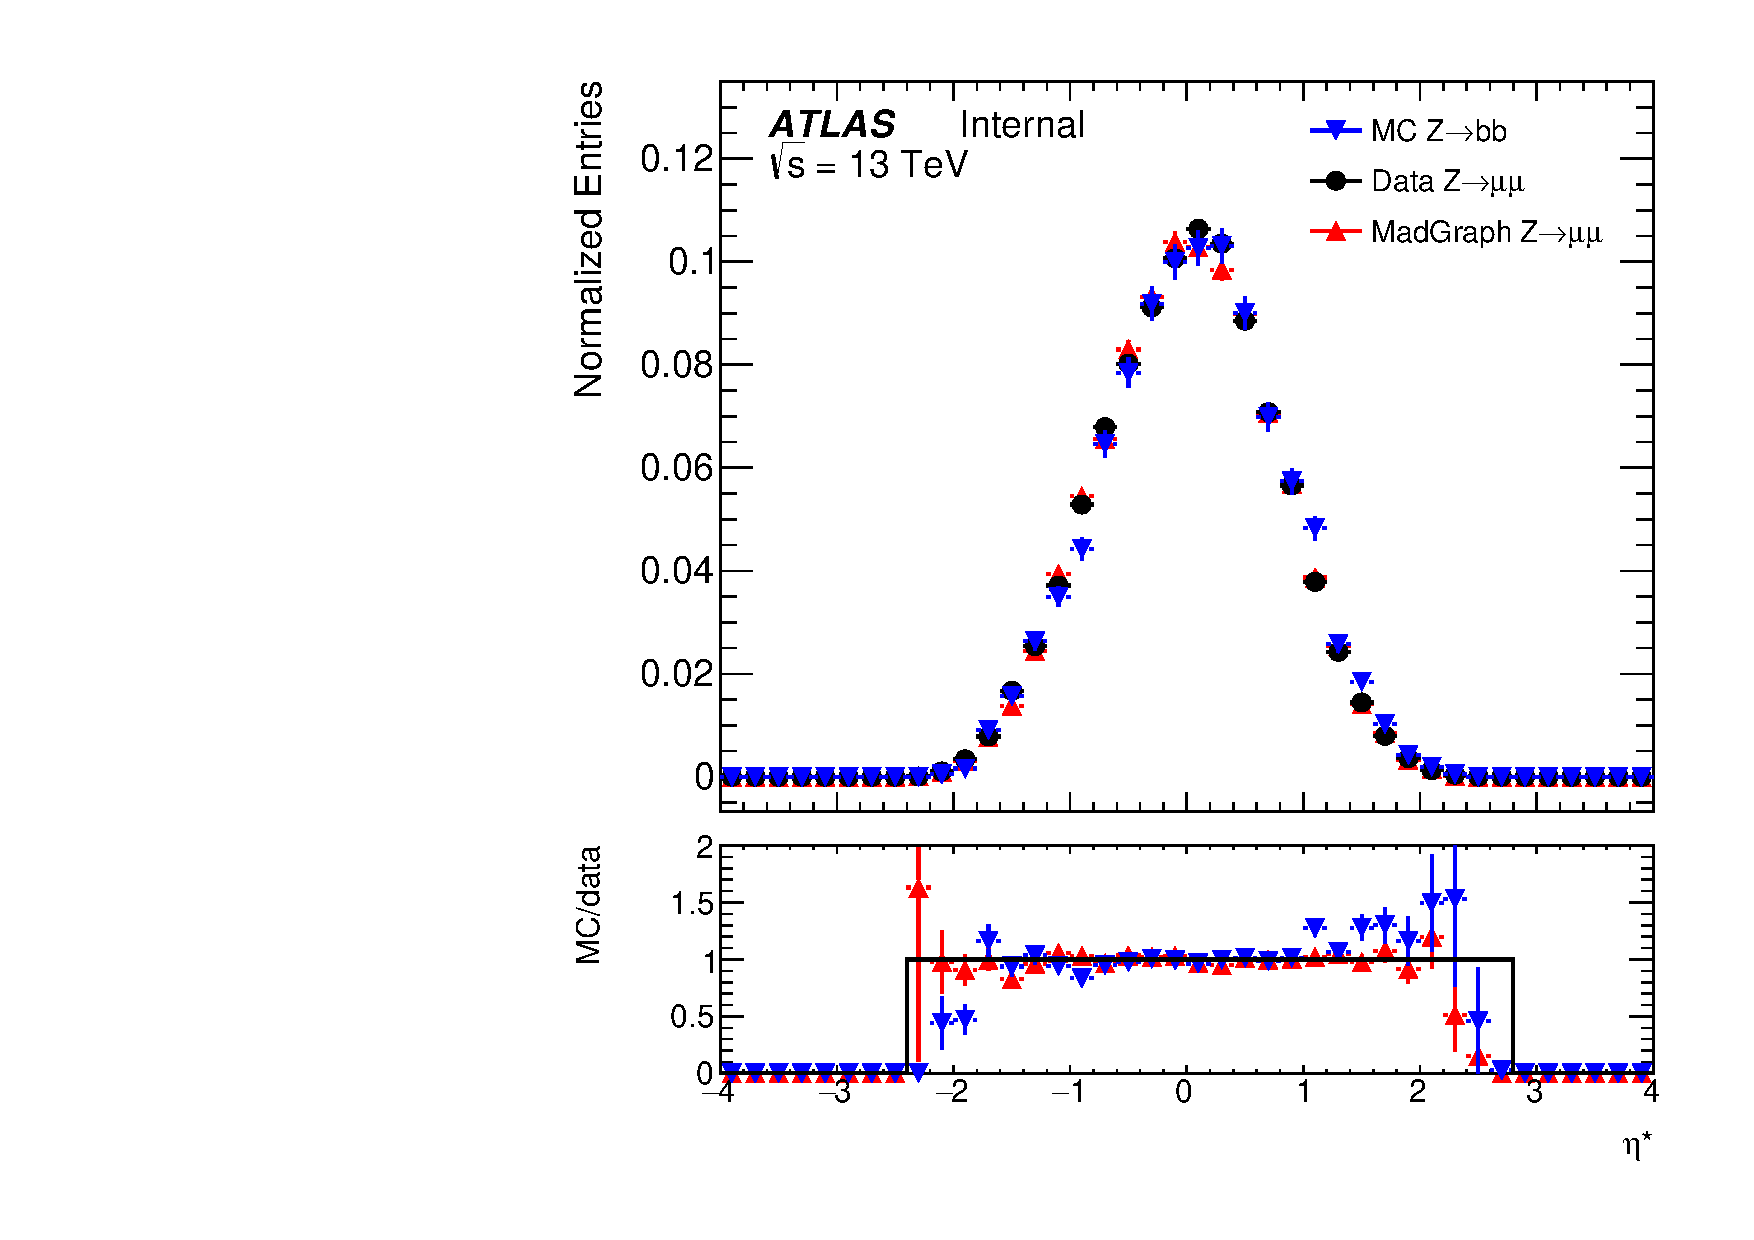
\includegraphics[width=0.3\textwidth]{figures/Zmumu/BDTinput_heta_J_star.pdf}\\
 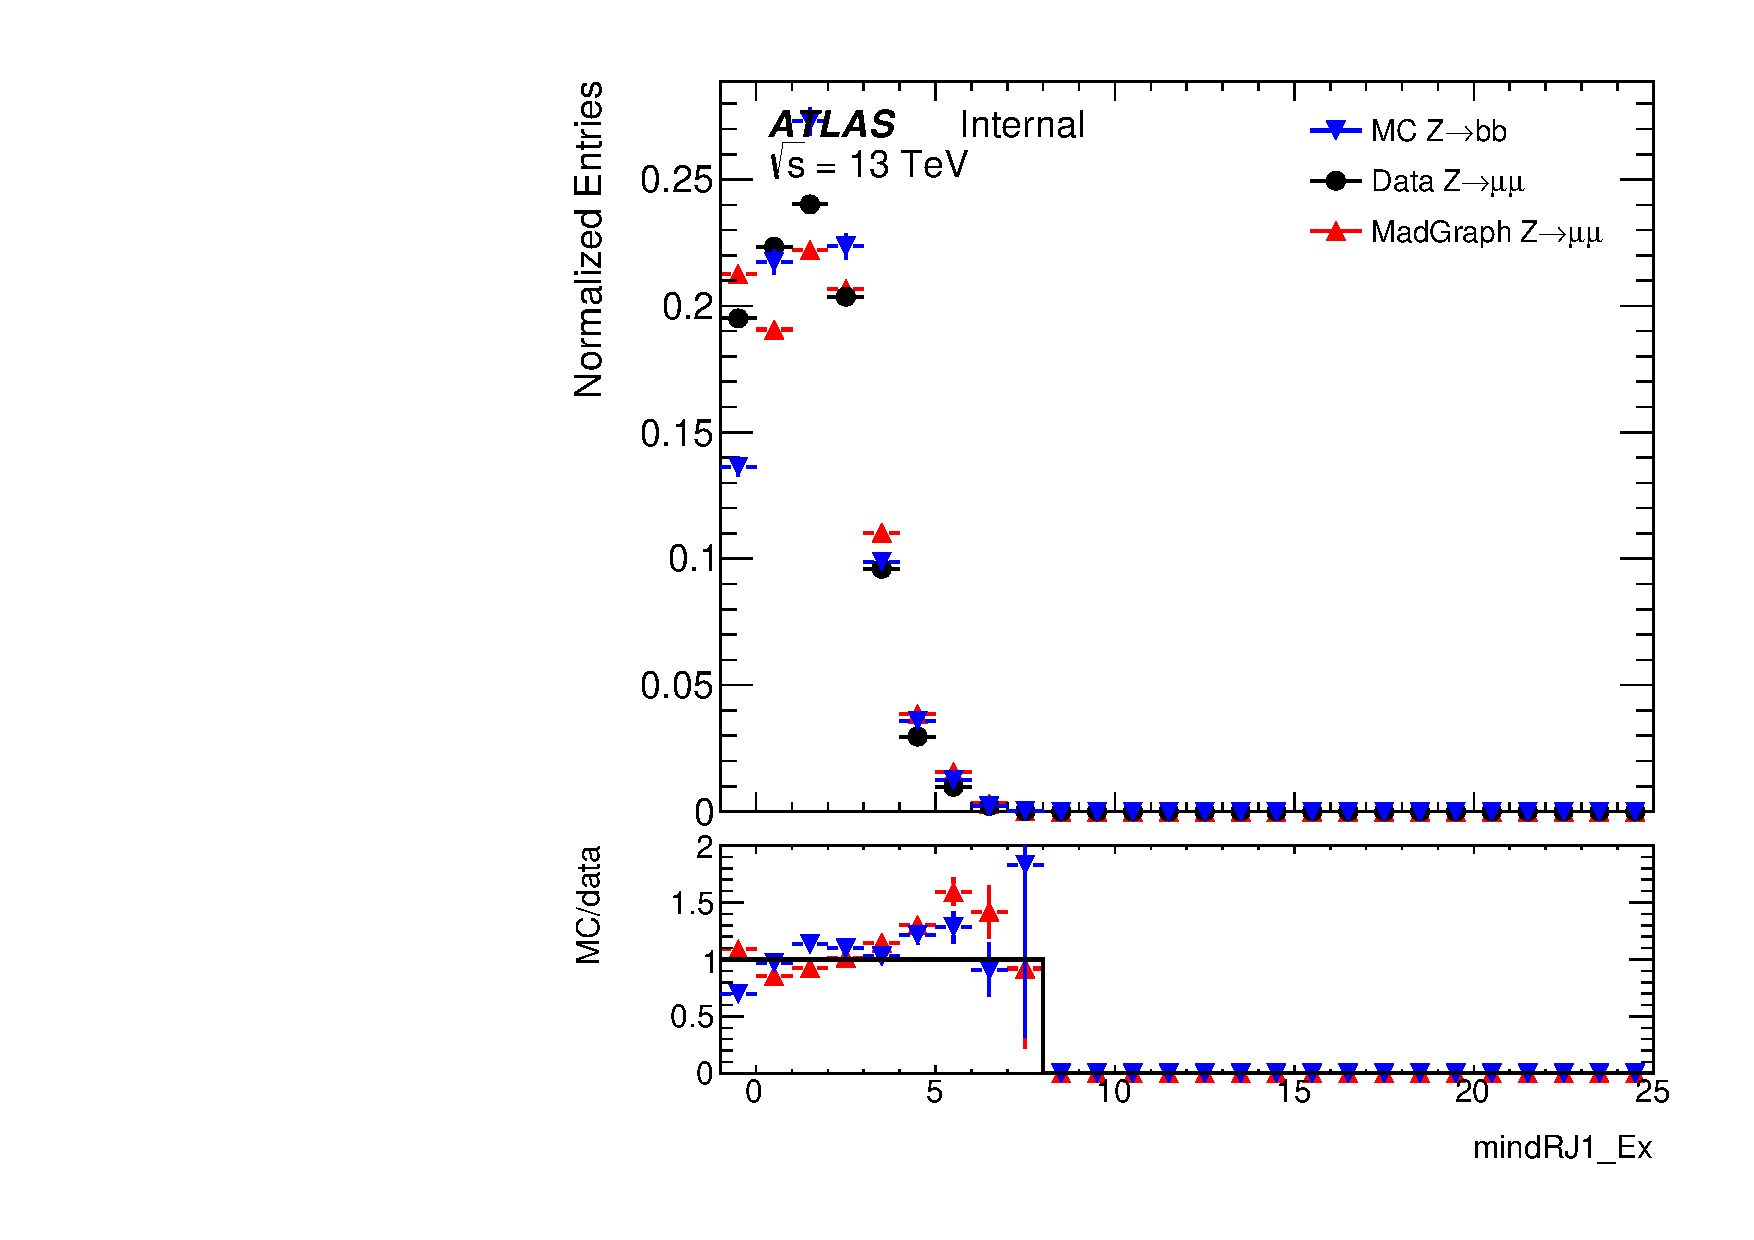
\includegraphics[width=0.3\textwidth]{figures/Zmumu/BDTinput_hmindRJ1_Ex.pdf}
 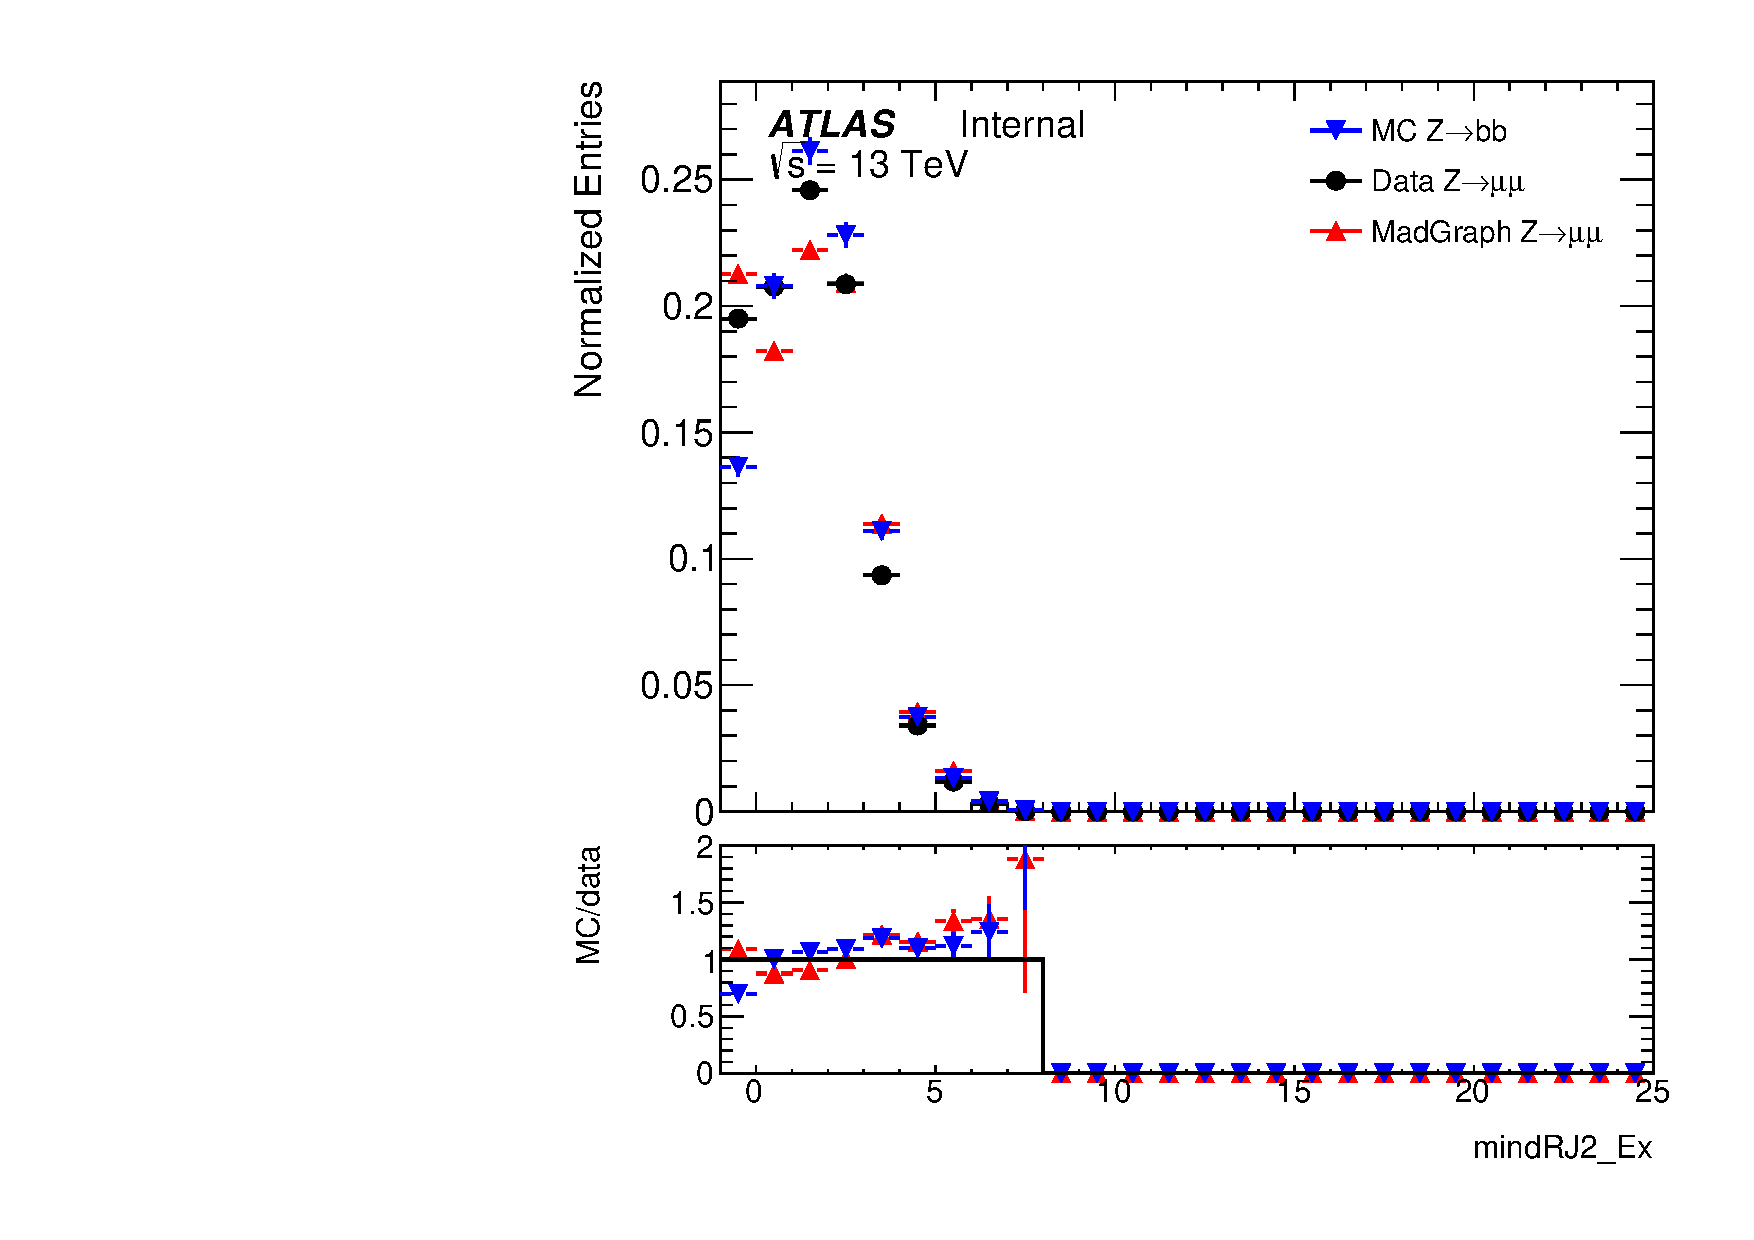
\includegraphics[width=0.3\textwidth]{figures/Zmumu/BDTinput_hmindRJ2_Ex.pdf}
 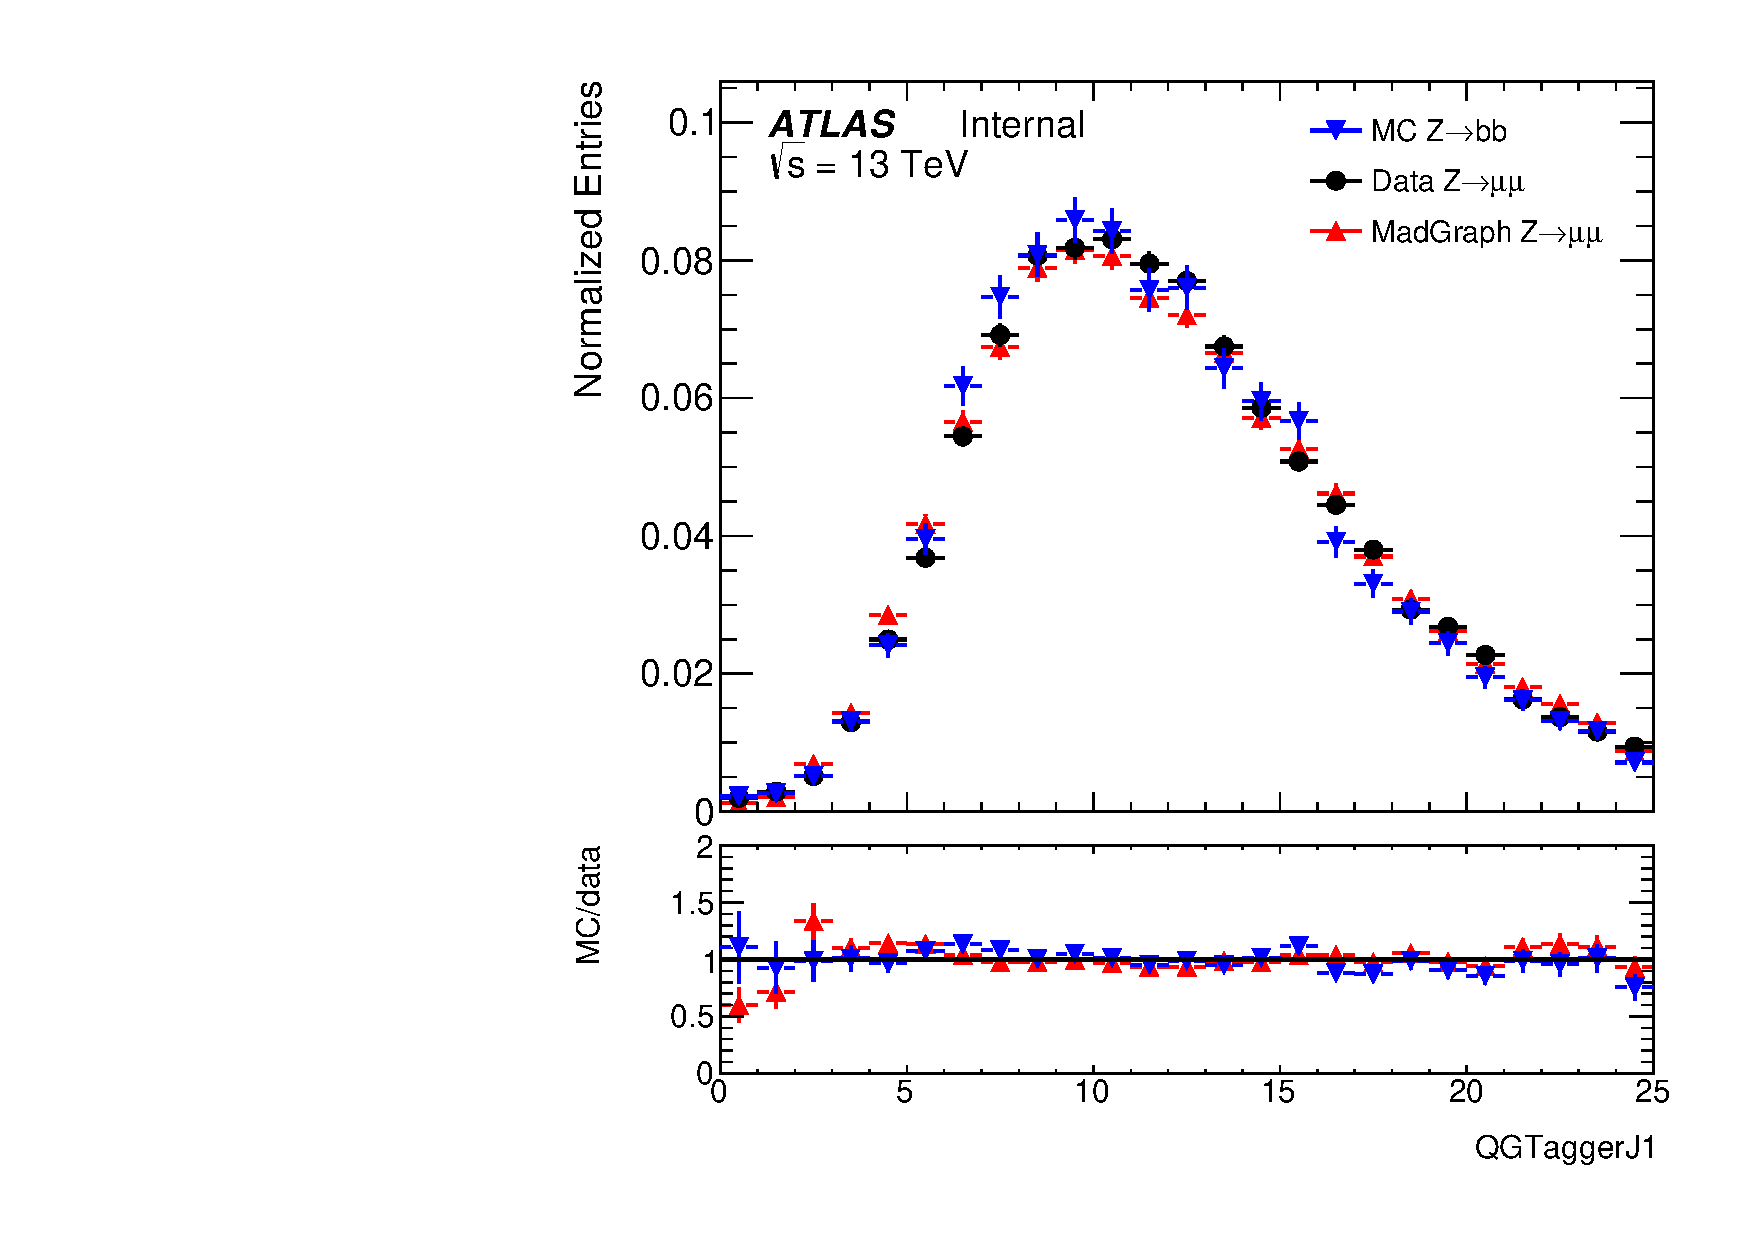
\includegraphics[width=0.3\textwidth]{figures/Zmumu/BDTinput_hQGTaggerJ1.pdf}\\
 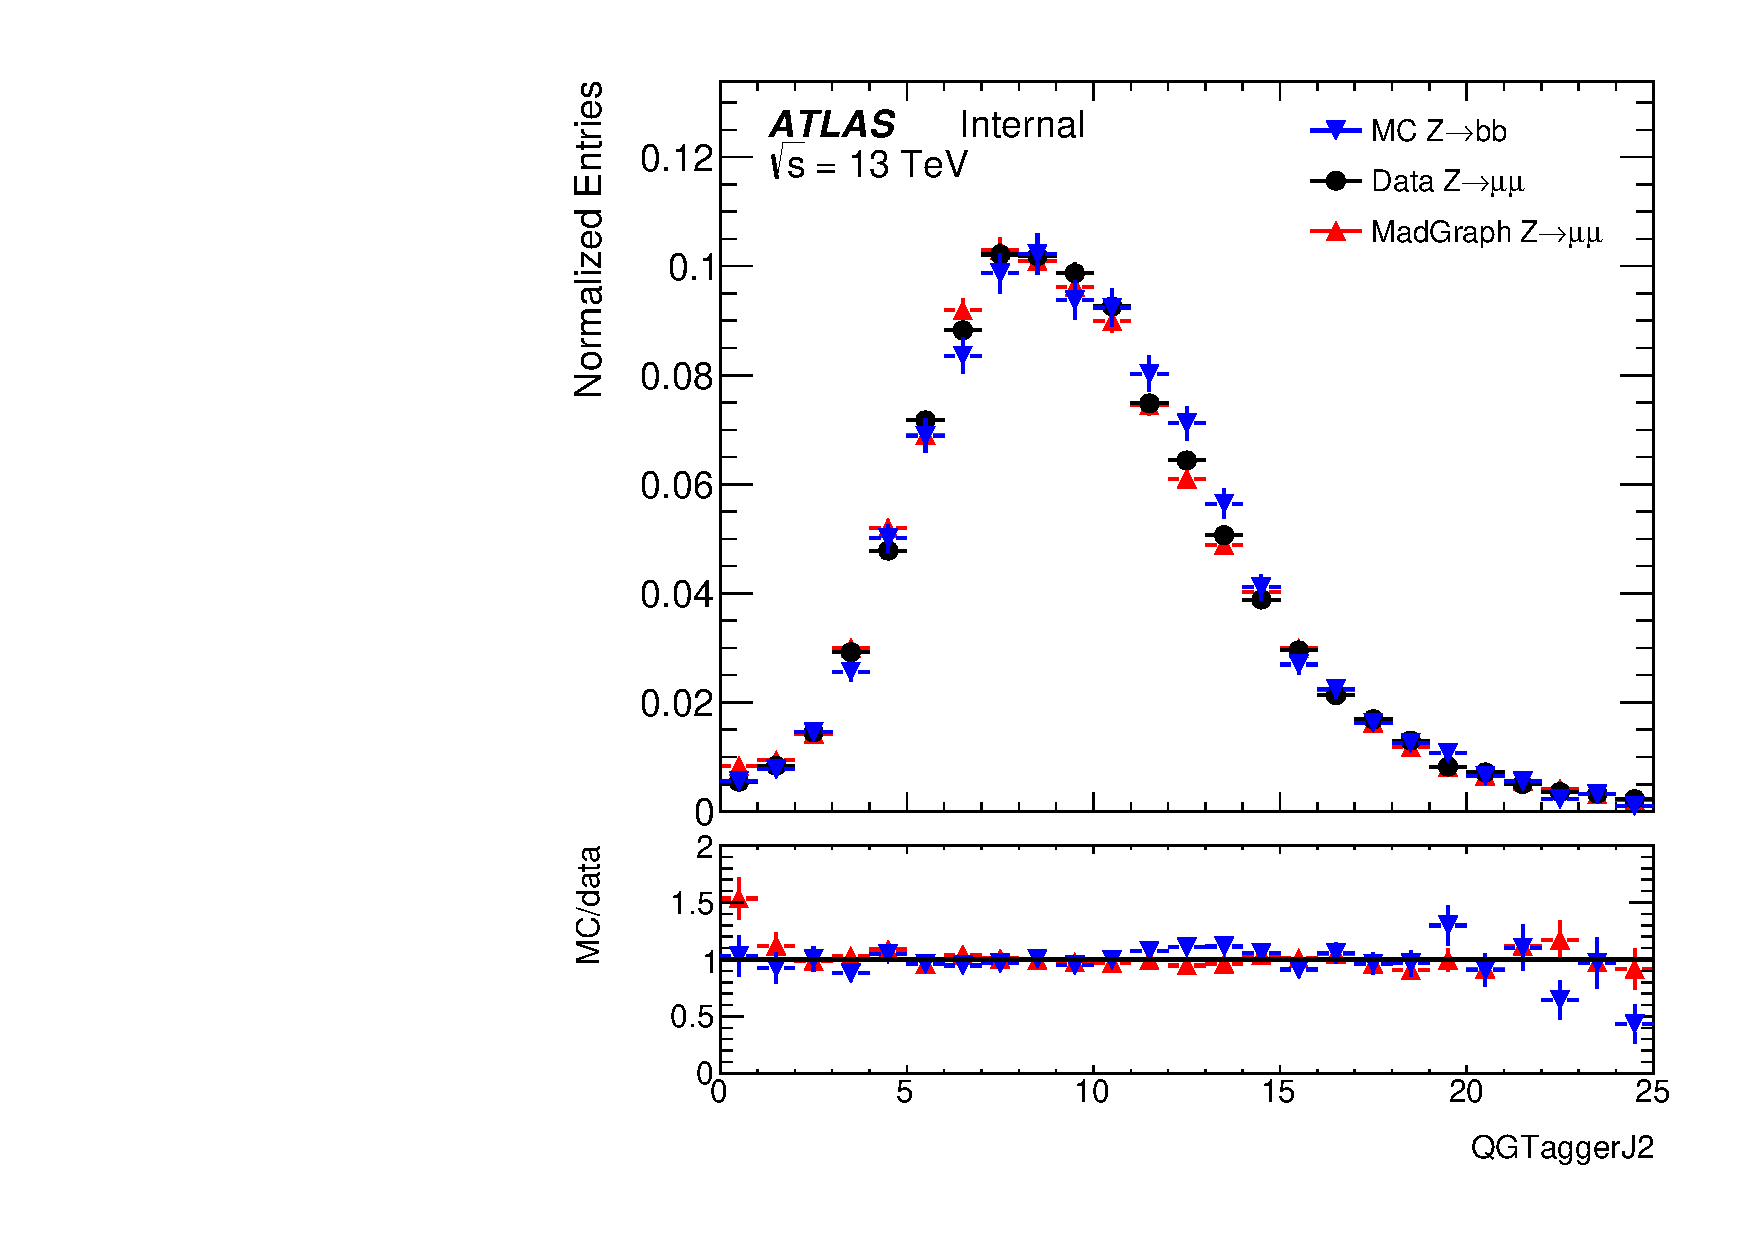
\includegraphics[width=0.3\textwidth]{figures/Zmumu/BDTinput_hQGTaggerJ2.pdf}
 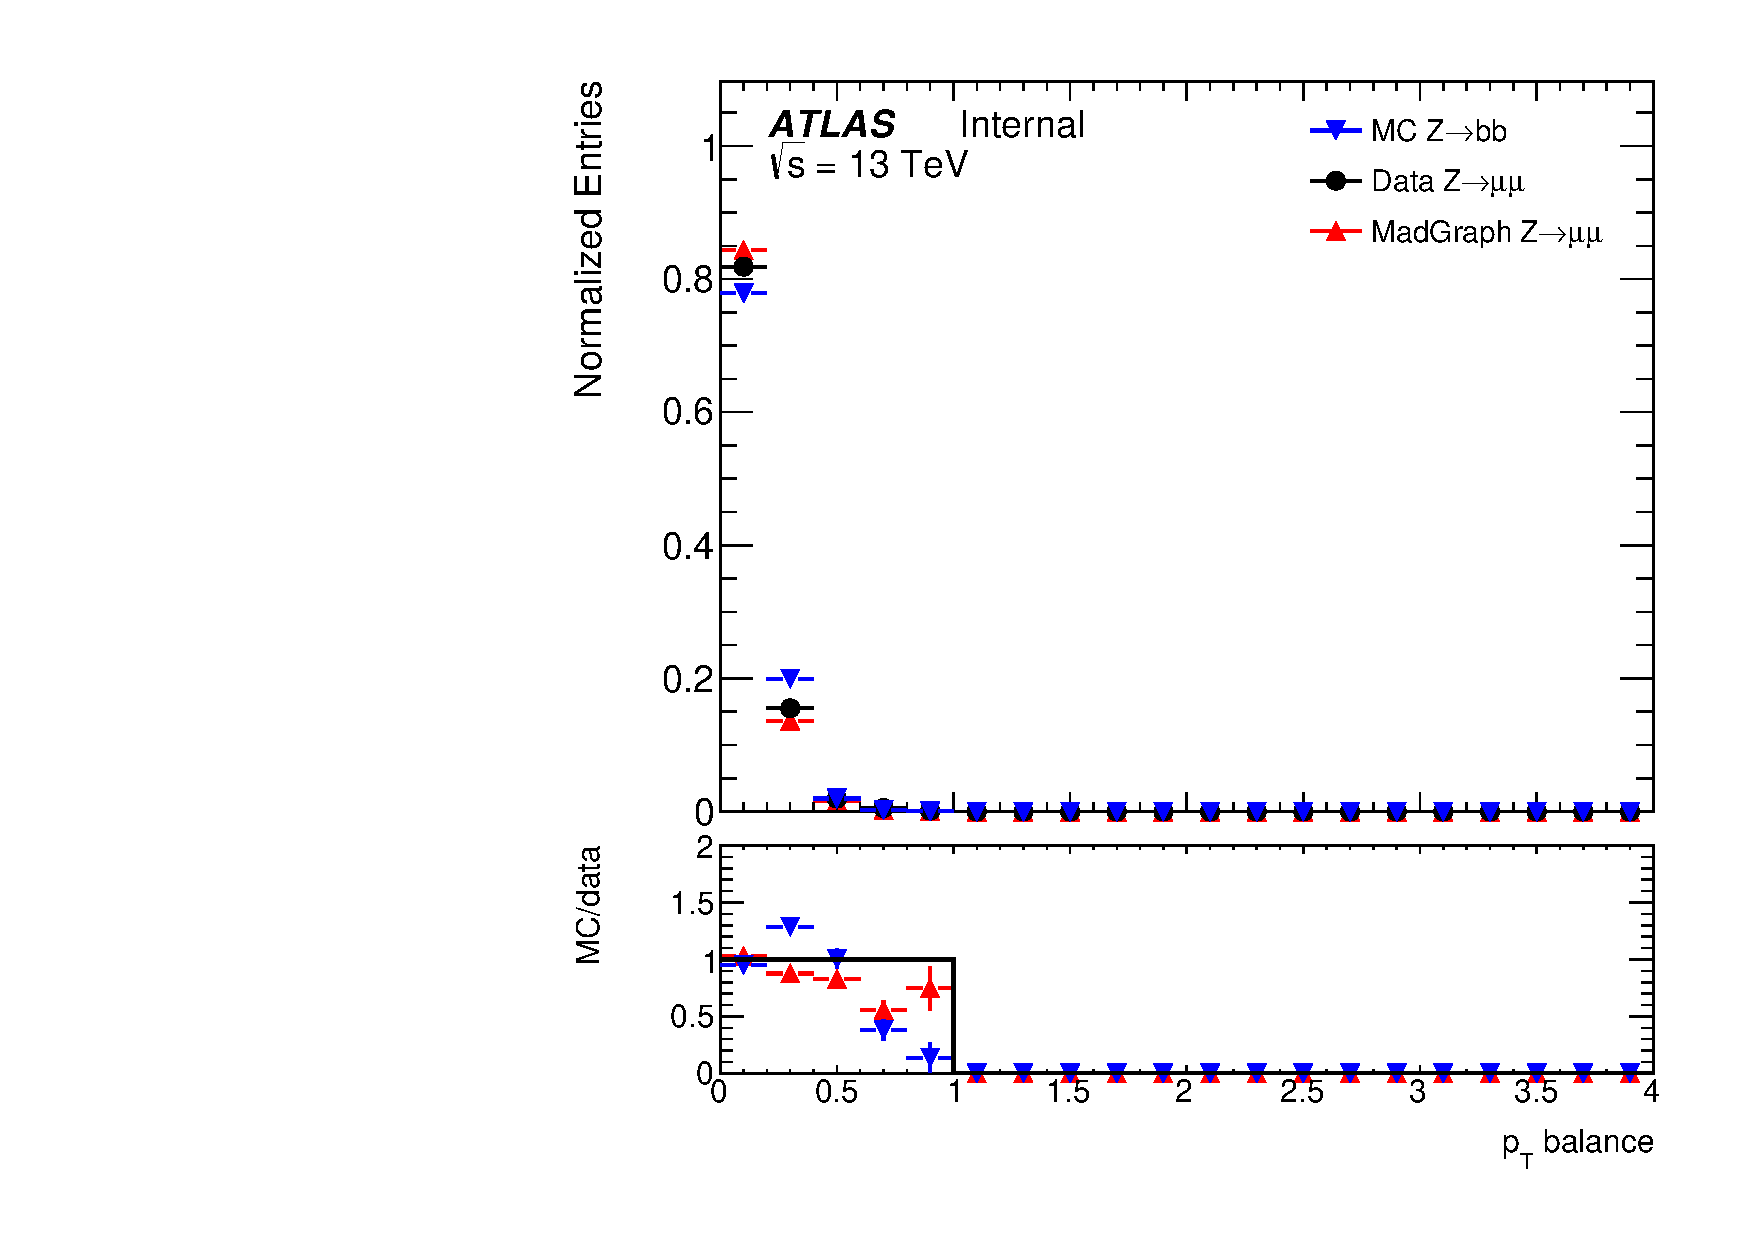
\includegraphics[width=0.3\textwidth]{figures/Zmumu/BDTinput_hpT_balance.pdf}\\
\caption{Distributions of BDT input variables of \fourcentral channel. }
  \label{fig:ZmmBDTInputs4cen}
\end{figure}

\begin{figure}[htbp]
  \centering
 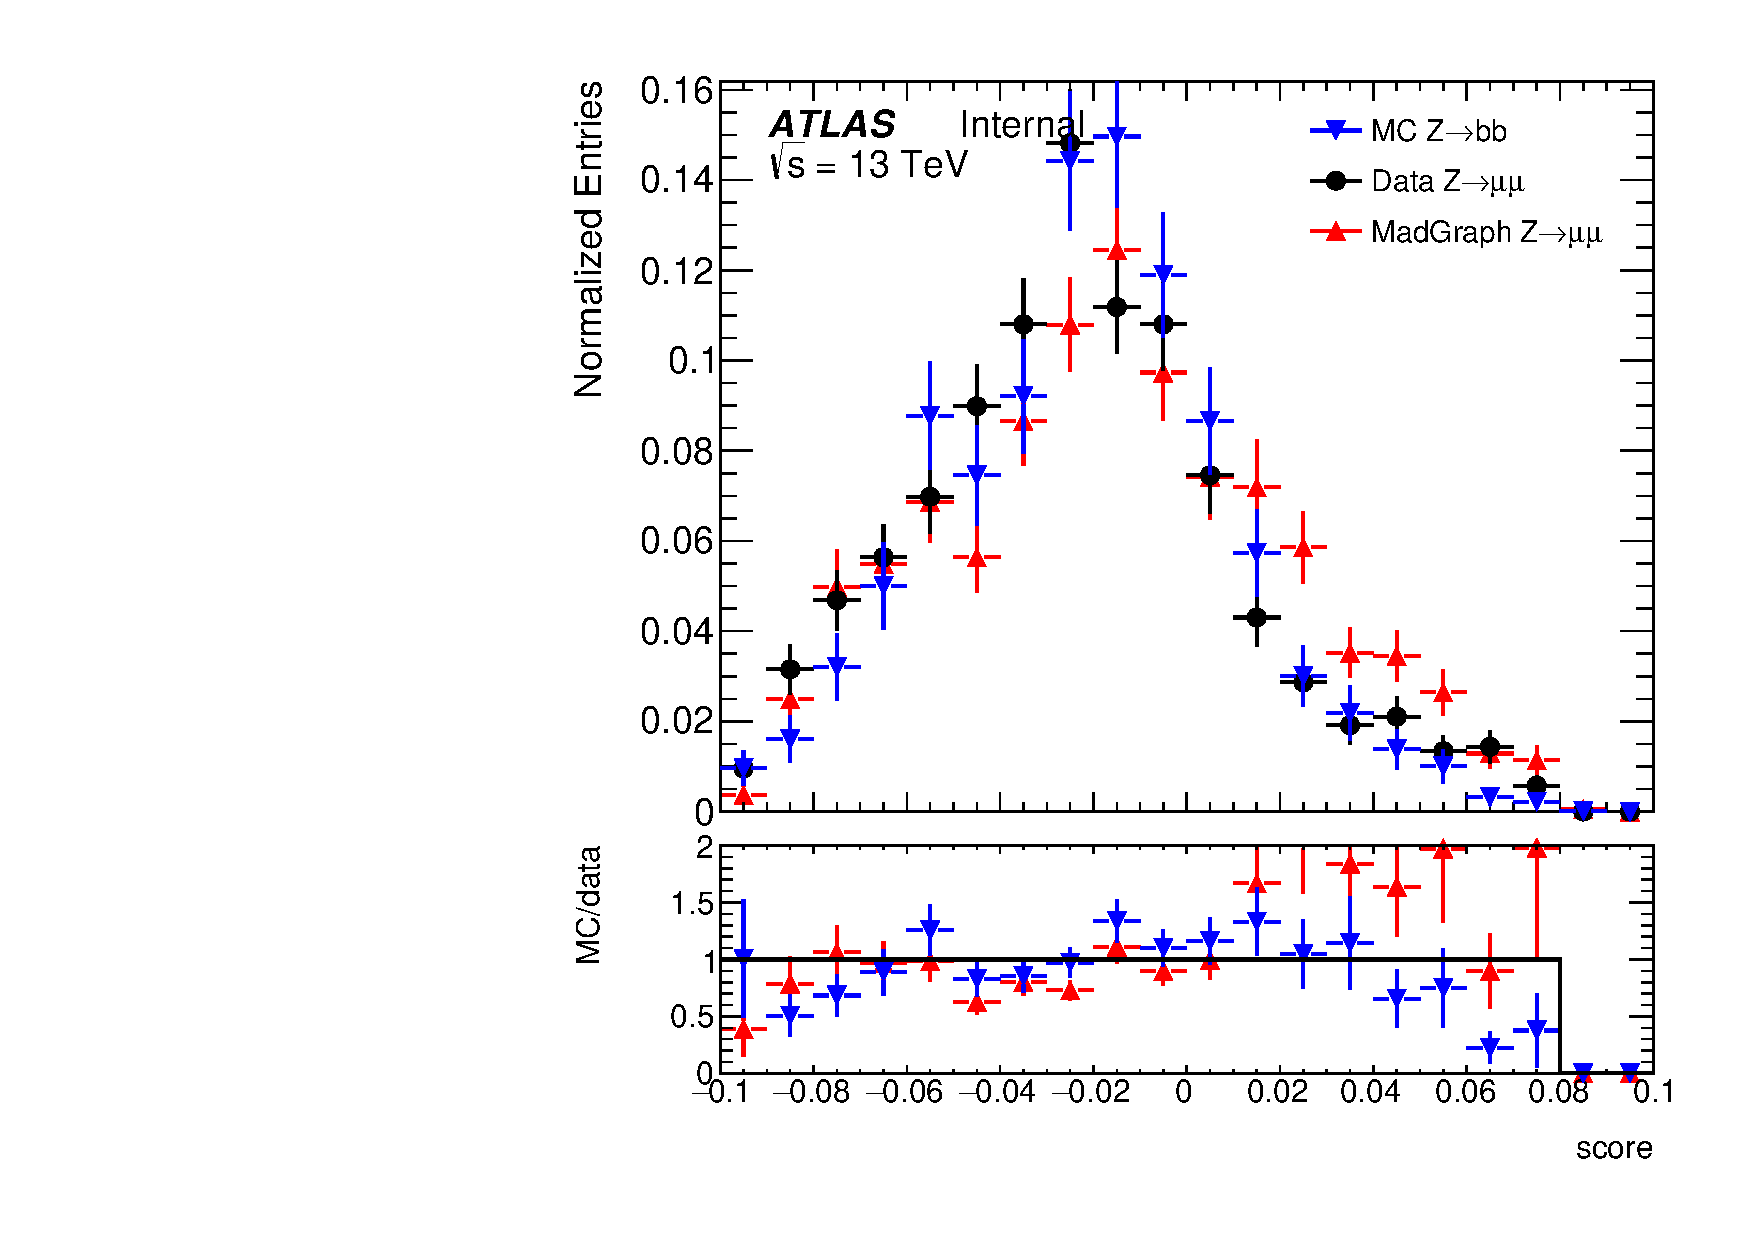
\includegraphics[width=0.3\textwidth]{figures/Zmumu/BDTinput_2j_hbdt.pdf}
 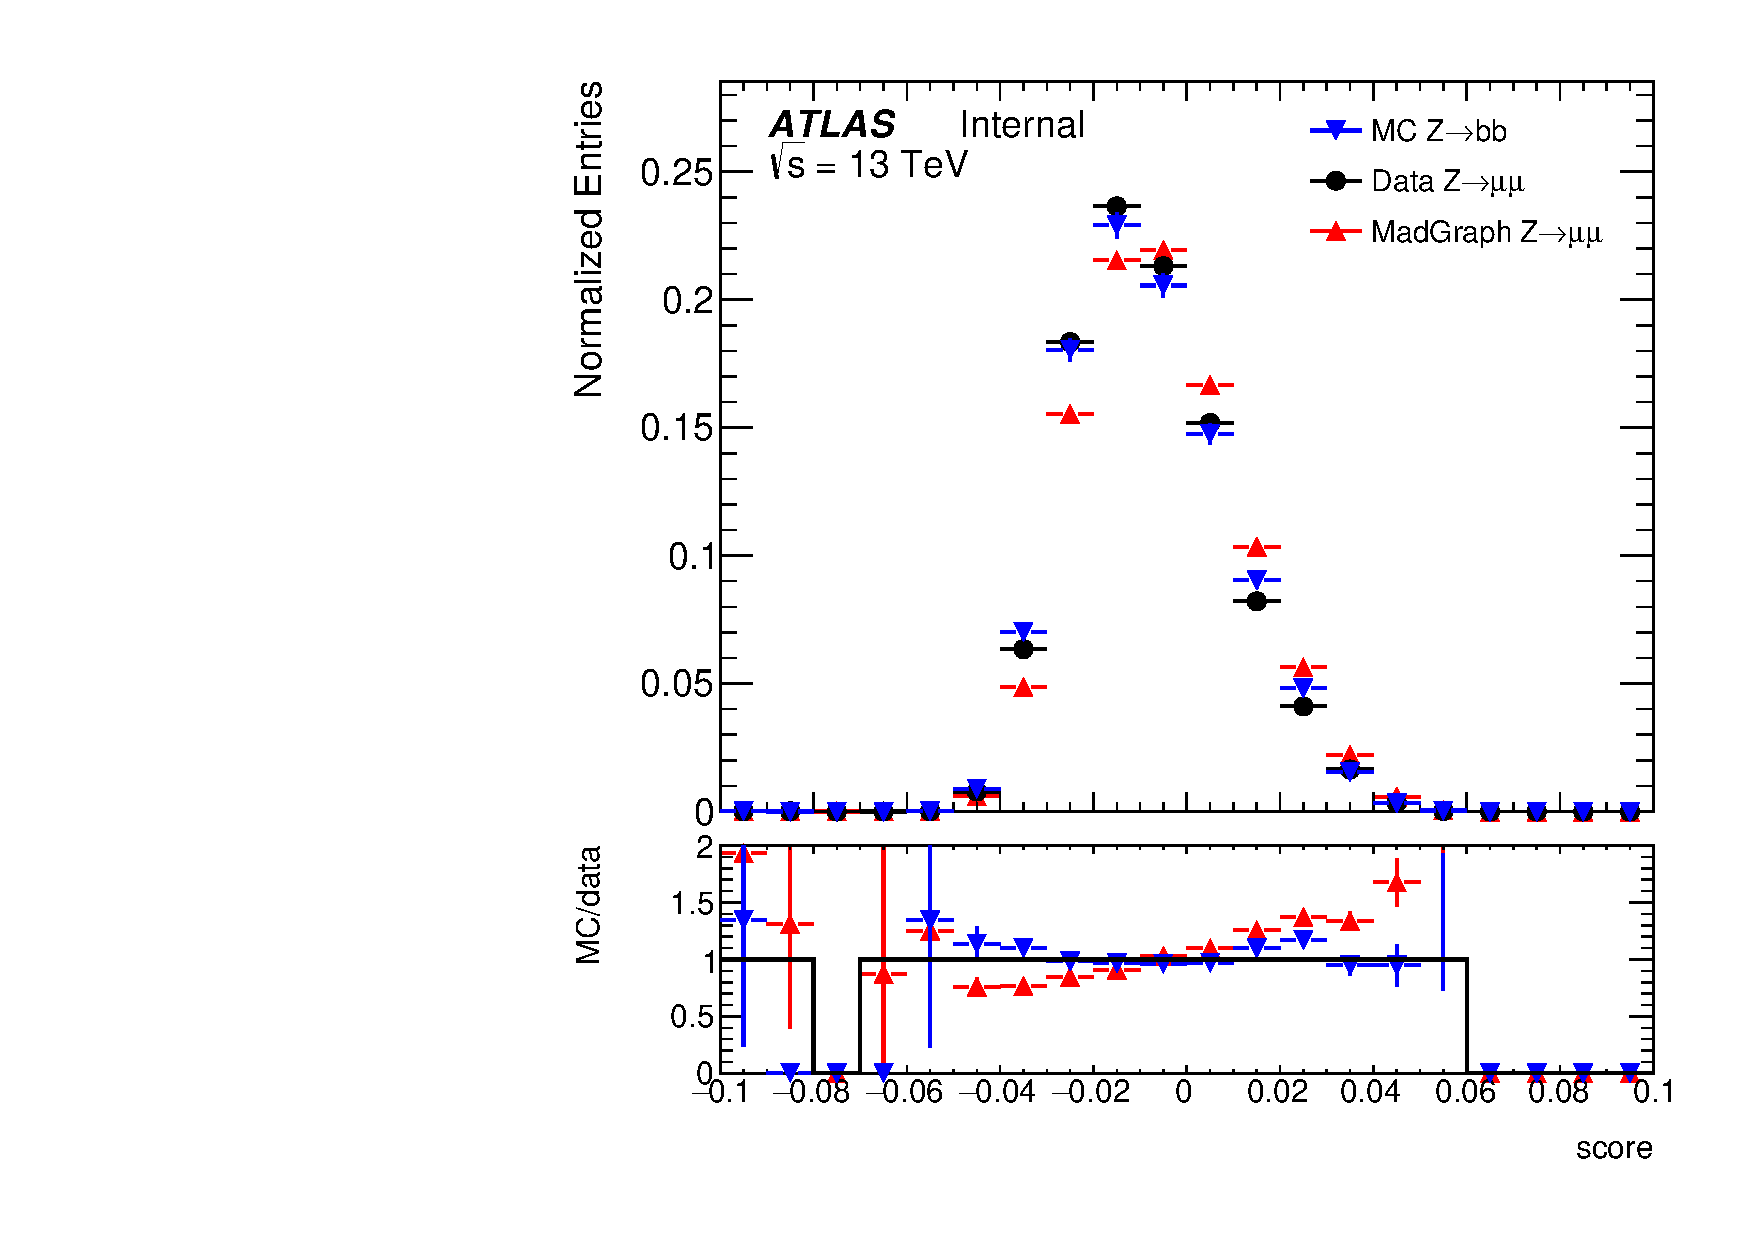
\includegraphics[width=0.3\textwidth]{figures/Zmumu/BDTinput_hbdt.pdf}
\caption{Distributions of BDT score for the \twocentral channel (left) and \fourcentral channel (right)}
  \label{fig:ZmmBDTInputsScore}
\end{figure}


%\begin{table}[]
%\centering
%\caption{Relative Ratios of $Z\rightarrow \mu \bar \mu$(Data) to \zjets{}(MC) in each BDT region}
%\label{tab:z_ratios}
%\begin{tabular}{|l|r|r|}
%\hline
%Region       &  $\frac{Z\rightarrow \mu \bar \mu(Data)}{Z\rightarrow \mu \bar \mu(MC)}$ & $\frac{Z\rightarrow b \bar b(MC)}{Z\rightarrow \mu \bar \mu(MC)}$   \\ \hline
%SRI (2cen)   & 0.82 (0.15) & 0.43 (0.12)\\ \hline
%SRII (2cen)  & 0.42 (0.13) & 0.35 (0.14)\\ \hline
%SRIII (2cen) & 0.61 (0.11) & 0.91 (0.17)\\ \hline
%CR (2cen)    & 1.26 (0.11) & 1.26 (0.13)\\ \hline
%SRI (4cen)   & 0.74 (0.05) & 0.64 (0.07)\\ \hline
%SRII (4cen)  & 0.80 (0.03) & 0.86 (0.05)\\ \hline
%CR (4cen)    & 1.47 (0.07) & 1.40 (0.09)\\ \hline
%\end{tabular}
%\end{table}


\FloatBarrier
